% Options for packages loaded elsewhere
\PassOptionsToPackage{unicode}{hyperref}
\PassOptionsToPackage{hyphens}{url}
%
\documentclass[
]{article}
\usepackage{amsmath,amssymb}
\usepackage{iftex}
\ifPDFTeX
  \usepackage[T1]{fontenc}
  \usepackage[utf8]{inputenc}
  \usepackage{textcomp} % provide euro and other symbols
\else % if luatex or xetex
  \usepackage{unicode-math} % this also loads fontspec
  \defaultfontfeatures{Scale=MatchLowercase}
  \defaultfontfeatures[\rmfamily]{Ligatures=TeX,Scale=1}
\fi
\usepackage{lmodern}
\ifPDFTeX\else
  % xetex/luatex font selection
\fi
% Use upquote if available, for straight quotes in verbatim environments
\IfFileExists{upquote.sty}{\usepackage{upquote}}{}
\IfFileExists{microtype.sty}{% use microtype if available
  \usepackage[]{microtype}
  \UseMicrotypeSet[protrusion]{basicmath} % disable protrusion for tt fonts
}{}
\makeatletter
\@ifundefined{KOMAClassName}{% if non-KOMA class
  \IfFileExists{parskip.sty}{%
    \usepackage{parskip}
  }{% else
    \setlength{\parindent}{0pt}
    \setlength{\parskip}{6pt plus 2pt minus 1pt}}
}{% if KOMA class
  \KOMAoptions{parskip=half}}
\makeatother
\usepackage{xcolor}
\usepackage[margin=1in]{geometry}
\usepackage{graphicx}
\makeatletter
\def\maxwidth{\ifdim\Gin@nat@width>\linewidth\linewidth\else\Gin@nat@width\fi}
\def\maxheight{\ifdim\Gin@nat@height>\textheight\textheight\else\Gin@nat@height\fi}
\makeatother
% Scale images if necessary, so that they will not overflow the page
% margins by default, and it is still possible to overwrite the defaults
% using explicit options in \includegraphics[width, height, ...]{}
\setkeys{Gin}{width=\maxwidth,height=\maxheight,keepaspectratio}
% Set default figure placement to htbp
\makeatletter
\def\fps@figure{htbp}
\makeatother
\setlength{\emergencystretch}{3em} % prevent overfull lines
\providecommand{\tightlist}{%
  \setlength{\itemsep}{0pt}\setlength{\parskip}{0pt}}
\setcounter{secnumdepth}{5}
\newlength{\cslhangindent}
\setlength{\cslhangindent}{1.5em}
\newlength{\csllabelwidth}
\setlength{\csllabelwidth}{3em}
\newlength{\cslentryspacingunit} % times entry-spacing
\setlength{\cslentryspacingunit}{\parskip}
\newenvironment{CSLReferences}[2] % #1 hanging-ident, #2 entry spacing
 {% don't indent paragraphs
  \setlength{\parindent}{0pt}
  % turn on hanging indent if param 1 is 1
  \ifodd #1
  \let\oldpar\par
  \def\par{\hangindent=\cslhangindent\oldpar}
  \fi
  % set entry spacing
  \setlength{\parskip}{#2\cslentryspacingunit}
 }%
 {}
\usepackage{calc}
\newcommand{\CSLBlock}[1]{#1\hfill\break}
\newcommand{\CSLLeftMargin}[1]{\parbox[t]{\csllabelwidth}{#1}}
\newcommand{\CSLRightInline}[1]{\parbox[t]{\linewidth - \csllabelwidth}{#1}\break}
\newcommand{\CSLIndent}[1]{\hspace{\cslhangindent}#1}
\usepackage{setspace}
\usepackage{float}
\floatplacement{figure}{H}
\ifLuaTeX
  \usepackage{selnolig}  % disable illegal ligatures
\fi
\IfFileExists{bookmark.sty}{\usepackage{bookmark}}{\usepackage{hyperref}}
\IfFileExists{xurl.sty}{\usepackage{xurl}}{} % add URL line breaks if available
\urlstyle{same}
\hypersetup{
  pdfauthor={Daniel Bonfil},
  hidelinks,
  pdfcreator={LaTeX via pandoc}}

\title{\hfill\break
\hfill\break
Affective Judgements in Retrospective Voting:\\
The Role of Framing and the End Bias\\
\strut \\}
\usepackage{etoolbox}
\makeatletter
\providecommand{\subtitle}[1]{% add subtitle to \maketitle
  \apptocmd{\@title}{\par {\large #1 \par}}{}{}
}
\makeatother
\subtitle{\hfill\break
\hfill\break
FGV EBAPE\\
\strut \\
\strut \\
First Qualifying Examination\\
(Conceptual Paper)\\
\strut \\}
\author{Daniel Bonfil}
\date{2023-12-22}

\begin{document}
\maketitle

{
\setcounter{tocdepth}{2}
\tableofcontents
}
\newpage
\doublespacing

\hypertarget{abstract}{%
\subsection{Abstract}\label{abstract}}

This research explores how affective judgments---emotional ties and
sentiments towards political leaders---influence citizens' economic
evaluations of identified incumbents, particularly in retrospective
voting. Affective judgments can shape perceptions of political leaders,
influencing performance evaluations by associating leaders with good or
bad times, regardless of their direct responsibility. Retrospective
voting often involves assessing incumbents' past economic performance.
However, the end bias---voters' overemphasis on the last year of
economic growth relative to the previous three in a presidential
term---can distort their assessments. Previous work by Healy \& Lenz
(2014) shows that the effect of such myopic behavior can be reduced with
the provision of ``right'' information through yearly and cumulative
framing. This research challenges these conclusions, moving beyond
hypothetical scenarios to examine real economic data and the interplay
of affect and cognitive biases. Our central question is whether these
findings remain robust in more realistic conditions, where individuals
assess the performance of politicians toward whom they have already
developed affect. Through a survey experiment, we employ a sentiment
thermometer to measure participants' affective responses to presidents
and how framing conditions may lead to unintentional emphasis on
election-year economic growth rather than evaluating leaders evenly
throughout their terms.

\hypertarget{introduction}{%
\subsection{Introduction}\label{introduction}}

Retrospective voting, the process of assessing incumbents' past
performance, is particularly susceptible to the influence of biases,
unrelated events, and framing (Huber et al., 2012). Conventional
defenses of democratic accountability rely on the theory of
retrospective voting to suggest that citizens would behave rationally
based on recollections of incumbents' past performance, even in the
presence of limited information (Fiorina, 1981; Key, 1966). However,
based on Kramer (1971), Fair (1978), and Tufte (1978), research by Achen
\& Bartels (2004) challenges this notion, arguing that voters often make
retrospective voting decisions based on how they feel about recent
conditions and their susceptibility to manipulation by governments.

The evaluation of presidential performance plays a controversial role in
retrospective voting especially due to the inherent limitations of human
information-processing capacity (Simon, 1957) and the widespread use of
cognitive heuristics or mental shortcuts (Kahneman, 2011; Lau \&
Redlawsk, 1997). Affective judgments, or emotional ties and sentiments
towards political leaders, have been shown to shape perceptions of
political figures, influencing performance evaluations by associating
leaders with good or bad times, regardless of their direct
responsibility (Campello \& Zucco, 2022; Lodge \& Taber, 2013). In the
context of economic performance evaluations, the end bias, voters'
myopic behavior that causes overemphasis on election-year economic
conditions, can lead voters to overweigh the last year of economic
growth relative to the previous three in a presidential term (Healy \&
Lenz, 2014). These findings suggest that affective judgments can play a
significant role in influencing retrospective voting decisions, leading
to potentially unfair and inaccurate economic performance evaluations of
incumbents.

The present research aims to build on findings by Campello \& Zucco
(2022) that demonstrate how individuals' prior affective ties to
political leaders cloud their willingness and capacity to accurately
apply available information, thereby affecting their ability to update
judgments of political figures. Healy \& Lenz (2014) showed that the
provision of appropriate information reduces individuals' myopic
behavior, yet they tested this effect with unidentified presidents.
Considering that prior affect color political judgments (Lodge \& Taber,
2013), we replicate the experiment by Healy \& Lenz (2014) but add
another treatment to account for the influence of affect. This will
involve presenting participants with real economic data where
individuals assess the performance of politicians for whom they may have
already developed affect.

Our main hypothesis is that the results found by Healy \& Lenz (2014)
may not hold with real politicians towards whom respondents have prior
affect. In this case, affect drives evaluations, and there will be no
relevant difference in judgments, regardless of whether individuals
focus on election-year or cumulative economic performance. We test this
by randomly assigning participants in our study to one of four distinct
conditions resulting from two manipulations. The framing manipulation
will involve presenting participants with real economic data framed
either at the yearly level (control condition) or at both the yearly and
cumulative levels (treatment condition). The affective manipulation will
involve presenting participants with real economic data for either an
unidentified incumbent (blind condition) or an identified incumbent
(identified condition).

This matters because economic voting can promote accountability, yet
this does not happen as voters display myopic behavior. This research
has implications for our understanding of how citizens evaluate
political leaders and make voting decisions. On the one hand, framing
economic information may have a limited impact on voter myopia that
Healy \& Lenz (2014) assume from their results. On the other hand,
framing economic information could be a valuable tool for reducing the
influence of affective judgments and promoting more accurate and fair
evaluations of incumbents. This research also has implications for the
design of news media campaigns and the development of more effective
communication strategies by government statistical agencies.

The remainder of the article is structured as follows. Section (3) and
(4) introduces notions of bounded rationality, heuristics, the surge of
dual-process models, and framing. Alongside, we explain the relationship
between the use of yearly and cumulative economic information, the end
bias, and the implications of framing and affective judgements. Section
(5) describes the experimental design and data, followed by the
hypotheses, and expected results in Section (6). Next, we interpret and
explain the main results of the online experiments in Section (7)
{[}TBD{]}, followed by the implications, limitations, and future
research possibilities in Section (8) {[}TBD{]}. Finally, concluding
remarks and applications are provided in Section (9) {[}TBD{]}.

\hypertarget{literature-review}{%
\subsection{Literature Review}\label{literature-review}}

Previous research by Healy \& Lenz (2014), examined the role of framing,
or the selection and presentation of information, in mitigating the end
bias, a myopic tendency for voters to weigh recent economic conditions
more heavily when evaluating incumbents. Their findings suggest that
framing economic information with both yearly and cumulative levels can
reduce the end bias, indicating that framing can help voters make more
balanced and informed retrospective assessments. However, this research
used hypothetical economic data and has not specifically addressed the
influence of affective judgments on retrospective voting.

Along with framing economic information, it is crucial to understand the
influence of affective judgments in evaluating identified incumbents.
Campello \& Zucco (2022) emphasize the issue of misattribution of
responsibility, which occurs when voters attribute economic conditions
to incumbents even when those conditions are determined by factors
beyond governmental control. They show that misattribution is not solely
a matter of access to information, but rather that voters often struggle
to accurately apply available information. They find that individuals'
prior affective ties to political leaders cloud their willingness and
capacity to discount exogenous conditions and therefore to update their
judgments of political figures.

In addition, Campello \& Zucco (2022) find that individuals are more
likely to use information to discount exogenous conditions and update
their judgments, particularly in the case of a hypothetical rather than
an identified incumbent. Their findings imply that updates are even less
likely when information is provided only one time as in their
experimental setting, which reinforces the pessimistic perspective of
Huber et al. (2012) on the effectiveness of information provision in
modifying individual behavior. These arguments contrast with Lodge \&
Taber (2013), who suggest that people automatically update their
attitudes toward a variety of social and political objects at the time
they encounter relevant information.

Affective ties pose a barrier to the objective evaluation of available
information and the updating of judgments especially when they clash
with affect for political figures (Campello \& Zucco, 2022). However,
the magnitude of exogenous factors varies significantly among regions,
generating positive or negative affective judgments that may be more
difficult to reverse in some countries compared to others. Notably, the
study by Healy \& Lenz (2014) focuses on the USA while research by
Campello \& Zucco (2022) is based in Brazil, where external factors
might exert a stronger influence on affective judgments.

Campello \& Zucco (2020) claim that exposure to exogenous shocks,
strongly associated with dependence on commodities and variations in
trade, is a fundamental structural difference between developed and
developing economies. They argue that countries highly exposed to
volatile exogenous conditions face more challenges in identifying the
competence of governments based on the economy. Finally, they suggest
that misattribution appears not to be just a problem of information
provision but rather a cognitive issue, and that the processing of
relevant information could allow for a better attribution of
responsibility for the economy in developed countries than in developing
ones.

Consequently, our research aims to determine whether the findings by
Healy \& Lenz (2014) which, in the context of economic evaluations where
framing can mitigate the influence of the end bias, hold in more
realistic conditions with the presence of affective judgments. As Lodge
\& Taber (2013) argue, affective judgments are activated faster than any
other consideration, and often operate unconsciously. This means that
voters may have already formed affective judgments about an incumbent's
economic performance based on recollections of particularly good or bad
economic conditions, without fully considering the incumbent's overall
record. Moreover, Taber and Lodge indicate that affective judgments are
closely linked to long term memory (LTM). This means that once voters
have formed an affective judgment about an incumbent, it can be very
difficult to change their minds, even in the face of contrary evidence.

Heuristics, or mental shortcuts, aid individuals to process information
and improve decision-making, especially due to the real-time limitations
of conscious processing (Redlawsk \& Lau, 2013; Taber \& Young, 2013).
While adaptive and efficient, they can also lead to biases and errors in
judgment (Kuklinski \& Quirk, 2000; Tversky \& Kahneman, 1974). For
instance, the ``end heuristic'' can lead to the end bias in various
contexts from undergoing colonoscopies (Redelmeier \& Kahneman, 1996) to
watching TV ads (Baumgartner et al., 1997). Similarly, the ``affect
heuristic,'' also referred to as the ``likeability heuristic,''
automatically links positive or negative emotions to familiar social
objects in LTM, potentially leading to motivated reasoning. Motivated
reasoning is a rationalization process driven by unconscious affective
biases, such as disconfirmation bias and active counterarguing (Taber \&
Young, 2013).

Lau \& Redlawsk (1997) suggest that the use of cognitive heuristics
seems a reasonable strategy to the extent that it helps align voters'
interests and values with candidates' positions and attributes. By
presenting voters with a more comprehensive picture of the incumbent's
economic performance, we hope to override the influence of affective
judgments and encourage voters to make more balanced and informed
evaluations. To test this hypothesis, we will conduct a survey
experiment where we will randomly assign participants to one of four
experimental conditions. Participants in the identified conditions will
first complete a sentiment thermometer to measure their affective
judgments towards each president included in the experiment. This will
allow us to assess whether affective judgments are driving their
evaluations of the incumbent's economic performance.

The proposed framing manipulation aligns with the affect-driven
dual-process theory of motivated reasoning proposed by Lodge \& Taber
(2013). This theory suggests that voters have two distinct modes of
thinking: an unconscious, automatic mode ``System 1'' and a conscious,
deliberative mode ``System 2''. Affective judgments are more likely to
influence voters when they are thinking in automatic mode. By framing
economic growth in a way that engages the conscious, deliberative mode,
we hope that participants use and process information to evaluate
incumbents even in the presence of prior affective judgements and the
challenges to update them.

To this end, we replicate the experiment by Healy \& Lenz (2014), but
add another treatment to account for the influence of prior affect. The
first manipulation for framing will involve presenting participants with
real economic data framed at either the yearly level (control condition)
or both the yearly and cumulative levels (treatment condition). This
manipulation will allow us to examine whether framing economic
information in a way that emphasizes both yearly and cumulative
performance helps participants to consider the entire term of an
incumbent, rather than just the election year. The second manipulation
will involve presenting participants with real economic data for either
an unidentified incumbent (blind condition) or an identified incumbent
(identified condition). This manipulation will allow us to assess the
impact of affective judgments on participants' evaluations.

\hypertarget{theoretical-framework}{%
\subsection{Theoretical Framework}\label{theoretical-framework}}

\hypertarget{heuristics-and-bounded-rationality}{%
\subsubsection{Heuristics and Bounded
Rationality}\label{heuristics-and-bounded-rationality}}

Traditional economic models of human decision-making have assumed
perfect rationality, portraying individuals as fully informed, perfectly
logical, and utility-maximizing agents (Chong, 2013; Neumann \&
Morgenstern, 2007). However, this idealized view has been challenged by
emerging perspectives that acknowledge the limitations of human
cognition and the influence of psychological factors on decision-making.

Herbert Simon's concept of bounded rationality marked a significant
departure from the traditional notion of perfect rationality.
Recognizing that individuals operate under constraints of information,
time, and processing power, Simon (1957) proposed that decision-making
is often bounded by these limitations, leading to strategies that are
satisficing rather than optimal. This concept challenged the assumptions
of Rational Choice Theory (RCT), suggesting that decisions are often
made using heuristics, mental shortcuts that allow for quick and
efficient decision-making, but can also lead to biases and suboptimal
outcomes.

The paradox of voting, identified by Anthony Downs, provides a
compelling illustration of the shortcomings of RCT. Downs (1957) argued
that the expected benefits of voting, such as influencing the outcome of
an election, are often outweighed by the costs involved, such as the
time and effort required to vote, and inform oneself about candidates
and issues. Despite this, voting remains a common practice, suggesting
that individuals may make decisions based on factors beyond
self-interest and rational calculations.

Behavioral decision theory (BDT) emerged as a response to the
limitations of RCT, recognizing the influence of psychological factors,
such as emotions, cognitive biases, and social influences, on
decision-making (Redlawsk \& Lau, 2013). A central concept in BDT is the
use of heuristics, which allow individuals to navigate complex
decision-making situations and reach satisficing rather than
value-maximizing results without requiring extensive deliberations
(Kahneman, 2003). These heuristics, while often adaptive and efficient,
can lead to systematic biases and errors in judgment (Tversky \&
Kahneman, 1974).

The concept of bounded rationality and the use of heuristics are
particularly relevant in the context of political decision-making. Faced
with an overwhelming amount of information about candidates, policies,
and political issues, voters often rely on heuristics to make informed
choices (Kuklinski \& Quirk, 2000). Heuristics such as party
identification, candidate endorsements, and incumbency advantage can
provide useful shortcuts, allowing voters to make judgments quickly and
efficiently. However, these heuristics can also lead to biases and
suboptimal outcomes. For instance, voters may rely too heavily on party
identification, leading to partisan biases that may not reflect their
preferences (Lau \& Redlawsk, 2001).

Prospect theory, developed by Kahneman \& Tversky (1979), further
highlights the limitations of human decision-making. This theory
suggests that individuals are more sensitive to losses than to gains,
leading to risk-averse behavior in the domain of gains and risk-seeking
behavior in the domain of losses. This bias can explain seemingly
irrational behavior, such as individuals rejecting a fair bet with an
equal chance of winning or losing a small amount of money but accepting
the same bet when the potential loss is framed as a gain.

Despite their potential pitfalls, heuristics play a crucial role in
human decision-making, allowing individuals to cope with information
overload and make choices in complex situations without requiring
extensive deliberation (Lau \& Redlawsk, 2001). In many cases,
heuristics can lead to satisfactory outcomes, particularly when the
costs of obtaining perfect information outweigh the potential benefits.
However, understanding the limitations of heuristics is essential for
making informed decisions. By recognizing the conditions under which
fast thinking, or System 1, can lead to errors, individuals can engage
in more deliberate, System 2 thinking, improving the quality of their
decisions (Kahneman, 2011).

\hypertarget{dual-process-models-and-rationalizers}{%
\subsubsection{Dual-Process Models and
Rationalizers}\label{dual-process-models-and-rationalizers}}

The recognition of the dual-process nature of human decision-making, as
proposed by Kahneman (2003), led to a surge in dual-process models in
various fields, including political psychology. Lodge \& Taber (2013)
adopted this framework to understanding political behavior, highlighting
the interplay between System 1, the fast, intuitive, and automatic
system, and System 2, the slow, deliberate, and effortful system. Within
our research, the concept of affective judgements, or rooted emotional
associations linked to political objects, play a crucial role in shaping
political preferences as they may limit voters' capacity to overcome
myopic behavior in the real world.

Moreover, Lodge \& Taber (2013) define the ``hot cognition hypothesis,''
which holds that all cognitive objects are linked to affective tags in
LTM via an associative network, and cannot be activated without
simultaneously activating their affective tags (Lodge \& Taber, 2005).
Motivated reasoning, a pervasive example of hot cognition, suggests that
we are motivated to maintain our existing beliefs and preferences,
sometimes at the expense of objective evaluation (Bartels, 1996). This
tendency can lead to biased interpretations of information, selective
recall of favorable evidence, dismissal of opposing viewpoints, the
overemphasis of confirming evidence, and the clinging to ideological
positions even in the face of overwhelming evidence to the contrary.

The System 1 likeability heuristic, proposed by Lodge \& Taber (2013),
guides candidate evaluations based on stored affective associations.
This heuristic operates through associative pathways, allowing rapid
activation of affective tags that automatically integrate and update
incoming information. The process of motivated reasoning is particularly
pronounced among individuals who have extensively considered political
figures, as they have developed stronger affective associations in LTM.
In contrast, those with less political interest and knowledge may not
have formed such strong affective associations, and therefore, may not
exhibit the same pattern of facilitation and inhibition that indicates
automatic affect. This highlights the role of individual differences in
political engagement in shaping the influence of affective judgments.

Affective judgments, intertwined with motivated reasoning, can cloud
objective assessments of political leaders and policies. Campello \&
Zucco (2022) research demonstrates that misattribution is not solely a
matter of access to information, but rather that voters often struggle
to accurately apply available information and update their judgements.
Specifically, they find that individuals' prior affective ties cloud
their capacity to discount exogenous conditions and hinder the objective
evaluation of available information especially when it clashes with
their affective judgments of political figures. This suggests that
affective judgments can significantly hamper the use of available
information hence, we are interested in whether different framing
conditions can help prevent the impairment of objective evaluation of
information.

\hypertarget{framing-friend-or-foe}{%
\subsubsection{Framing: Friend or Foe?}\label{framing-friend-or-foe}}

Framing, coupled with cognitive biases plays a pivotal role in shaping
citizens' responses to economic information. The nexus between
democratic accountability and framing dynamics holds significance as
political actors and media outlets strategically frame issues to shape
public opinion and perceptions of government performance (McCombs \&
Shaw, 1972). Framing's impact on public discourse and agenda-setting is
further complicated by its interaction with affective judgments,
scholars like Goffman (1986) and Lakoff (2014) argue that the way an
issue or message is framed can activate certain cognitive schemas and
influence how individuals understand and respond to it. Moreover, Marcus
et al. (2000) and Sniderman \& Theriault (2004) delve into how framing
shapes public opinion and behavior, influencing how citizens perceive
their representatives and how they hold them accountable.

Framing, or the selection and presentation of information, can
significantly influence individuals' preferences and choices, even when
the underlying facts remain the same (Druckman, 2001a). As Huber et al.
(2012) demonstrate, subtle framing manipulations can significantly alter
individuals' retrospective assessments. This underscores the potential
of framing to influence the way people evaluate and interpret
information as well as how they react to it.

Equivalence frames, logically equivalent but differently phrased
descriptions of the same issue, can lead to different decisions (Chong,
2013). For instance, the example by Kahneman \& Tversky (1979)
highlights the inconsistency of human decision-making as individuals
reversed their preferences when presented with options framed as gains,
people tended to make risk-averse choices, opting for the safer option
with a guaranteed outcome. However, when the same options were framed as
losses, people made risk-seeking choices, preferring the riskier option
with the potential to avoid a loss, even if it meant a higher chance of
incurring an even greater loss. Our take is that framing can serve as a
tool to address biases and sustain the effectiveness of heuristics.
Healy \& Lenz (2014) provide compelling evidence that even myopic
psychological biases can be overcomed when individuals have access to
pertinent information. Their study reveals that when voters are
presented with the attribute of total economic growth over a president's
term, they are better equipped to evaluate presidents based on their
overall performance, mitigating the influence of the end bias.

As Chong (2013) highlights, framing effects have a profound impact on
how individuals perceive and respond to political issues. However, the
mere presence of framing may not be sufficient to elicit rational
responses from citizens, particularly in the face of affective
judgments. Individuals vary in their susceptibility to framing effects,
influenced by factors such as cognitive ability, strong attitudes, and
the need to justify preferences (Druckman, 2001b). Those with stronger
attitudes or a higher need for cognitive consistency may be less
susceptible to framing.

In the upcoming sections, we offer a comprehensive overview of our
research design, building upon the previously presented foundational
insights and available data.

\hypertarget{research-design-and-data}{%
\subsection{Research Design and Data}\label{research-design-and-data}}

Our study builds upon the original data and experiment conducted by
Healy \& Lenz (2014), which explores the impact of framing yearly and
cumulative RDI growth rates on participants' economic evaluations while
addressing the end bias. We replicate and extend this experiment using
real economic data sourced from the Bureau of Economic Affairs (BEA).
Specifically, we use data from 17 US presidential tenures from 1940 to
2008, instead of the 25 hypothetical 4-year economies. The dataset
includes Real Disposable Income (\(RDI\)) with both yearly and
cumulative growth rates and the names of the respective presidents
during their terms. To delve into the effects of framing economic
information on mitigating the influence of affective judgments we align
with the approach advocated by Campello \& Zucco (2022), enabling us to
examine whether framing can indeed facilitate a more balanced and
informed assessment of the economic performance of identified
incumbents.

Experimental findings, as highlighted by Huber et al. (2012), reveal
participants' inclination to disproportionately emphasize recent
incumbent performance. Over a series of experiments, Healy \& Lenz
(2014) demonstrate that participants tend to overweight the last year's
performance, despite intending to weigh growth equally across all years.
Using the incumbent party's vote margin (\(incmargin\)) in 17 US
elections, they expose a noteworthy correlation (\(\rho = 0.734\)) with
participants' naïve economic evaluations (\(economy\)) and the
Election-Year Real Disposable Income (\(RDI_y\)) growth rate for each of
the four years, as shown in Figure 1 below. Furthermore, they show that
the end bias can be mitigated by providing voters with both yearly and
cumulative economic information. When both types of information are made
equally accessible, the election-year emphasis is eliminated, leading to
a more balanced and informed evaluation of incumbents' economic
performance.

\begin{figure}
\hypertarget{fig:label}{%
\centering
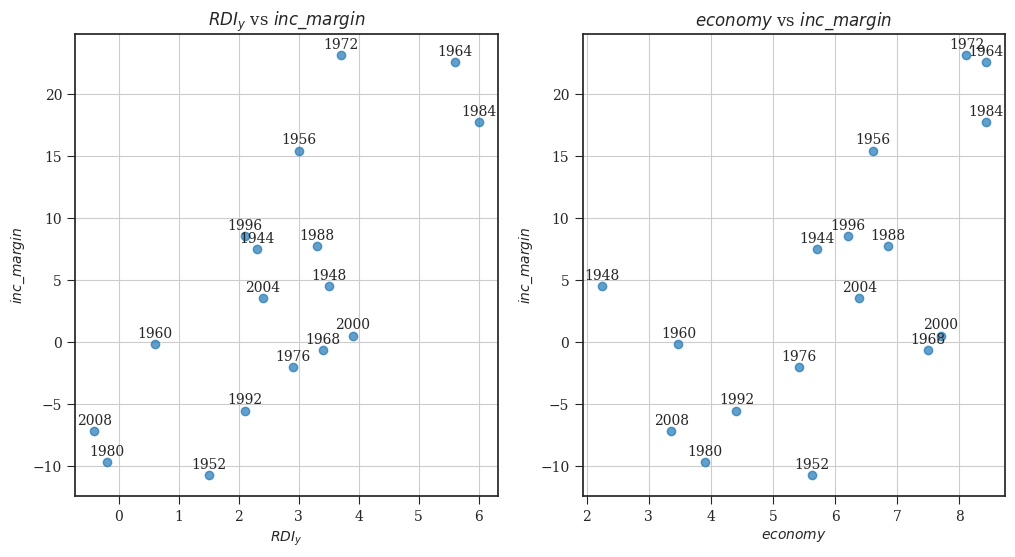
\includegraphics[width=0.9\textwidth,height=0.9\textheight]{C:/Users/danbo/OneDrive - Fundacao Getulio Vargas - FGV/FGV/Q3.23/GIT/GIT/incmarg.png}
\caption{Vote Margin vs RDI Growth and Economic
Evaluations}\label{fig:label}
}
\end{figure}

To reinforce the previous plots, Table 1 below provides regression
results for both (\(incmargin\)) and (\(economy\)) with valuable
insights into the relationship between economic evaluations and voting
behavior in the context of 17 elections. To ensure comparability, both
the actual vote margin and economic evaluations were rescaled to vary
from 0 to 1 in Columns (3) and (4). The coefficients represent the
estimated impact of income growth in each year of presidents' terms on
the rescaled variables.

For (\(incmargin\)), the coefficients indicate the implicit weights each
year of income growth contributes to the incumbent party's actual vote
margin. Notably, the coefficient for (\(RDI_4\)) (Year 4) is the
highest, suggesting that the income growth in the fourth year has the
most substantial positive impact on the vote margin. The p-values from
the hypothesis tests further support the significance of the
coefficients, highlighting that income growth in the fourth year
significantly influences respondents' economic evaluations relative to
each of the previous years, with exception of year 3 that is only
statistically significant at the 10\% level.

Similarly, for (\(economy\)), the coefficients indicate the implicit
weights between income growth in each year and respondents' economic
evaluations. (\(RDI_4\)) again stands out with the highest coefficient,
indicating a pronounced impact on economic evaluations. The associated
p-values for the hypothesis tests comparing the coefficients for
(\(RDI_4\)) with other years are all statistically significant,
reinforcing the importance of the fourth year's income growth in
influencing voters' decisions.

\begin{center}
  \begin{table}[!htbp]
\centering
\caption{Economic Evaluations and Incumbent Margin vs RDI Growth}
\begin{tabular}{@{\extracolsep{2pt}}lcccc}
\\[-1.8ex]\hline
\hline \\[-1.8ex]
\\[-1.8ex] & \multicolumn{1}{c}{Economy} & \multicolumn{1}{c}{Vote Margin} & \multicolumn{1}{c}{Economy (Rescaled)} & \multicolumn{1}{c}{Vote Margin (Rescaled)}  \\
\\[-1.8ex] & (1) & (2) & (3) & (4) \\
\hline \\[-1.8ex]
 RDI\textsubscript{1} & -0.127$^{*}$ & -0.032$^{}$ & -0.020$^{*}$ & -0.001$^{}$ \\
& (0.061) & (0.700) & (0.010) & (0.021) \\
 RDI\textsubscript{2} & 0.159$^{**}$ & -0.425$^{}$ & 0.026$^{**}$ & -0.013$^{}$ \\
& (0.061) & (0.701) & (0.010) & (0.021) \\
 RDI\textsubscript{3} & 0.494$^{***}$ & 1.483$^{}$ & 0.080$^{***}$ & 0.044$^{}$ \\
& (0.081) & (0.937) & (0.013) & (0.028) \\
 RDI\textsubscript{4} & 0.812$^{***}$ & 4.368$^{***}$ & 0.131$^{***}$ & 0.129$^{***}$ \\
& (0.093) & (1.070) & (0.015) & (0.032) \\
 const & 2.866$^{***}$ & -8.448$^{**}$ & 0.101$^{*}$ & 0.068$^{}$ \\
& (0.330) & (3.817) & (0.053) & (0.113) \\
\hline \\[-1.8ex]
 Observations & 17 & 17 & 17 & 17 \\
 $R^2$ & 0.916 & 0.640 & 0.916 & 0.640 \\
 Adjusted $R^2$ & 0.888 & 0.520 & 0.888 & 0.520 \\
 Residual Std. Error & 0.634 (df=12) & 7.322 (df=12) & 0.102 (df=12) & 0.216 (df=12) \\
 F Statistic & 32.822$^{***}$ (df=4; 12) & 5.335$^{**}$ (df=4; 12) & 32.822$^{***}$ (df=4; 12) & 5.335$^{**}$ (df=4; 12) \\
\hline
\hline \\[-1.8ex]
\textit{Note:} & \multicolumn{4}{r}{$^{*}$p$<$0.1; $^{**}$p$<$0.05; $^{***}$p$<$0.01} \\
\end{tabular}
\end{table}
\end{center}

The observations from the original experiment suggest a consistent
pattern where the fourth year plays a substantial role in shaping both
the actual vote margin and economic evaluations. The similitudes between
real-world voting behavior and experimental responses enhance the
external validity of the findings, indicating that the experimental
results capture similar dynamics observed in actual elections.

\hypertarget{experimental-conditions}{%
\subsubsection{Experimental Conditions}\label{experimental-conditions}}

The experimental design, as illustrated in Figure 2, will be implemented
in Qualtrics for participants recruited from Amazon Mechanical Turk
(MTurk), drawing from a pool of US citizens. Participants will be
incentivized with a payment of \$0.25 US Dollars for their involvement
in the study. The survey begins with a consent and an attention screener
before engaging in economic evaluations across the different conditions.
Participants in the identified conditions respond a 7-point feeling
thermometer gauging respondents' sentiments toward political leaders.
The survey concludes with a brief demographic, ideological, and party
identification questionnaire.

\begin{figure}
\hypertarget{fig:label}{%
\centering
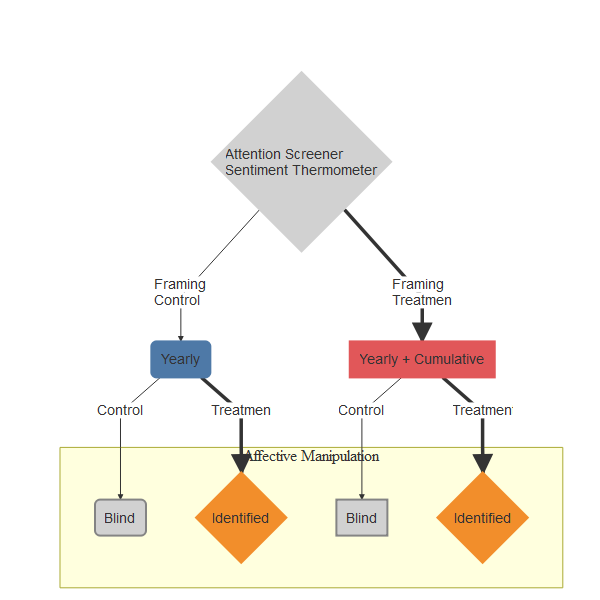
\includegraphics[width=0.5\textwidth,height=0.5\textheight]{C:/Users/danbo/OneDrive - Fundacao Getulio Vargas - FGV/FGV/Q3.23/GIT/GIT/expdesign2.png}
\caption{Experimental Design}\label{fig:label}
}
\end{figure}

Participants in our study will be randomly assigned to one of four
distinct conditions resulting of two manipulations. The framing
manipulation will involve presenting participants with real economic
data framed at either the yearly level (control condition) or both the
yearly and cumulative levels (treatment condition). This manipulation
will allow us to examine whether framing economic information in a way
that emphasizes both yearly and cumulative performance helps
participants to consider the entire term of an incumbent, rather than
just the election year. The affective manipulation will involve
presenting participants with real economic data for either an
unidentified incumbent (blind condition) or an identified incumbent
(identified condition). This manipulation will allow us to assess the
impact of affective judgments on participants' evaluations.

\begin{itemize}
\tightlist
\item
  In the Framing Manipulation, the Control Condition presents
  participants with yearly growth plots, resembling the top panel of
  Figure 3. In the Treatment Condition it exposed participants to both
  yearly and cumulative growth plots together, including the top and
  bottom panels of Figure 3. We display two presidential terms for
  illustration purposes but participants are only exposed to one term at
  a time (either left or right panels of Figure 3).
\end{itemize}

\begin{figure}
\hypertarget{fig:label}{%
\centering
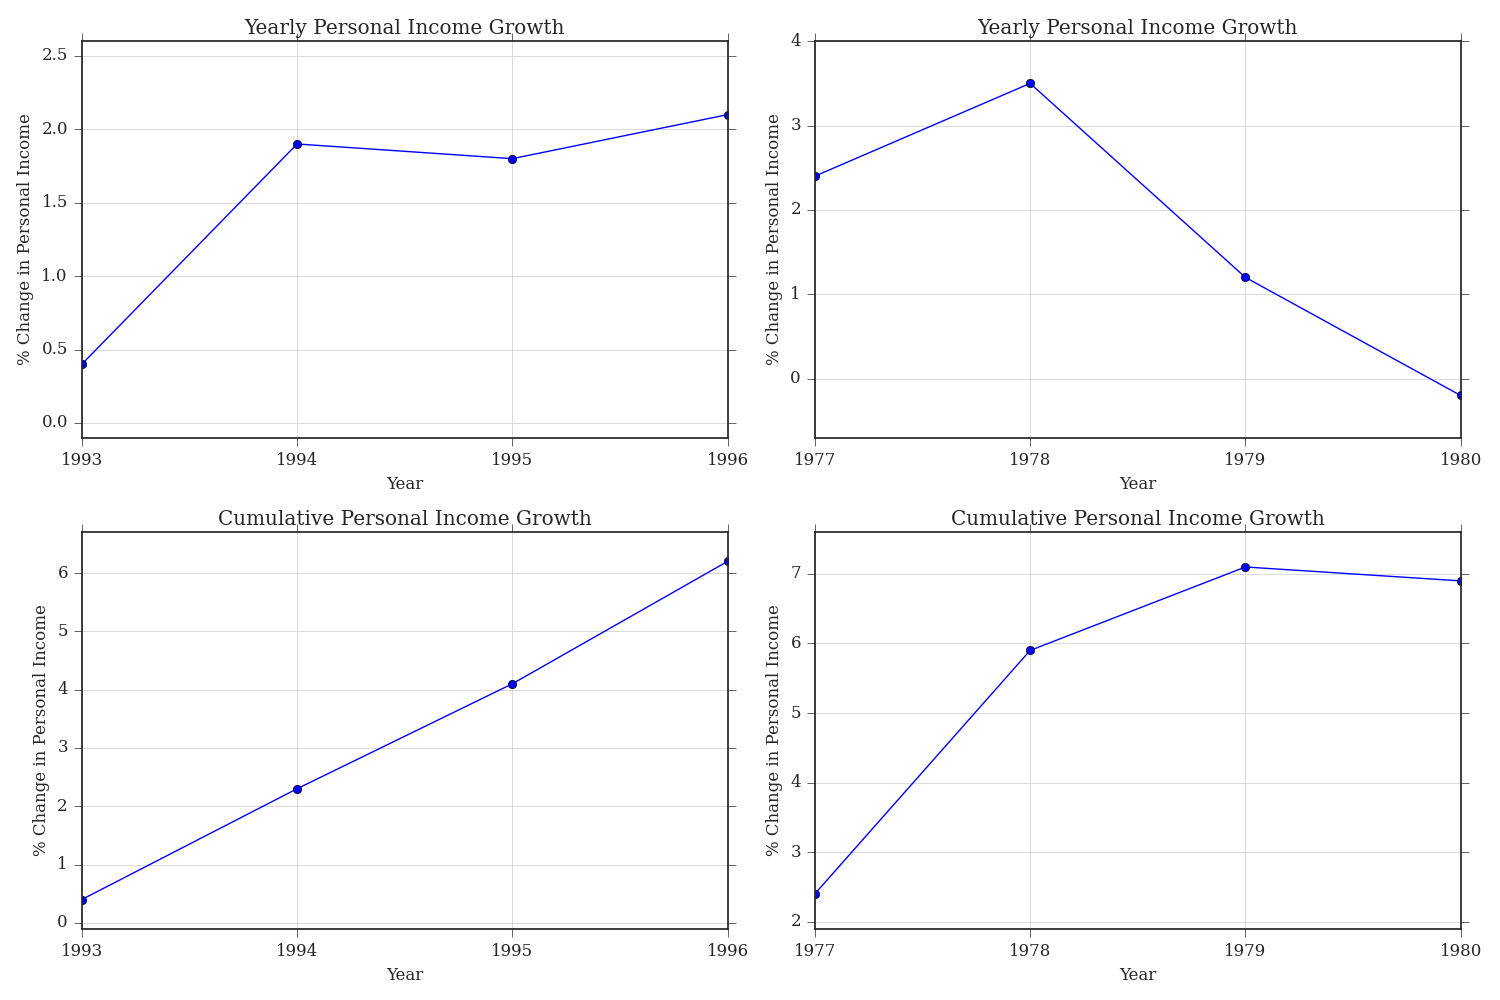
\includegraphics[width=0.9\textwidth,height=0.9\textheight]{C:/Users/danbo/OneDrive - Fundacao Getulio Vargas - FGV/FGV/Q3.23/GIT/GIT/clintoncarter_cum.png}
\caption{Framing Manipulation}\label{fig:label}
}
\end{figure}

\begin{itemize}
\tightlist
\item
  The Affective Manipulation featured the same graphs but revealed the
  names of presidents (Identified Condition) or without names (Blind
  Condition). These conditions allowe us to investigate the influence of
  different framing techniques and the impact of presidential
  identification on participants' economic evaluations.
\end{itemize}

Following the original experiment, after each plot we will ask ``How
would you rate the condition of the national economy during this period?
Is it very good, fairly good, fairly bad, or very bad?'' Responses will
be recorded to vary from 0 to 10, with 10 corresponding to ``very good''
in order to put RDI growth and economic evaluations on a similar scale.
Please refer to the Annex for details of the online survey.

Economic evaluations of Figure 3 clearly depict the pattern shown in
Figure 1 where, even when presented with data from all years of a
President's Term in a simple format, most participants placed
substantially more weight on the economy in the final year of
presidents' terms. For instance, consider the left panel, which
corresponds to Bill Clinton's initial term. It portrays a period of
moderate average growth, culminating in a notably strong phase. In
contrast, the right panel showcases Jimmy Carter's sole term,
characterized by more robust growth during the first two years, followed
by a marked deceleration in the election year. Interestingly, despite
the cumulative income growth being superior during Carter's tenure
(6.9\% compared to Clinton's 6.2\%), participants consistently evaluated
the economy more favorably during Clinton's first term (6.2 compared to
Carter's 3.9 on the 10-point scale). This striking phenomenon
underscores the prevalence of the end bias and its potential to
influence participants' economic evaluations, even when presented with
comprehensive data from all years of a presidential term.

\hypertarget{regression-analysis}{%
\subsubsection{Regression Analysis}\label{regression-analysis}}

To understand the influence of each year on participants' economic
evaluations, we will employ regression analysis. Specifically, we will
regress participants' average economic evaluations on the percentage
change in (\(RDI_y\)) growth for each of the four years within a
presidential term. This regression model is represented by Equation 1:
\[
(1) y_i = \beta_0 + \beta_1 X_1 + \beta_2 X_2 + \beta_3 X_3 + \beta_4 X_4 + \varepsilon_i
\] Where: - \(y_i\) represents the economic evaluation of participant
\(i\). - \(X_1, X_2, X_3,\) and \(X_4\) represent the (\(RDI_y\)) growth
rates for the four years of the presidential term. -
\(\beta_1, \beta_2, \beta_3,\) and \(\beta_4\) are coefficients
estimating the implicit weight assigned to each year. -
\(\varepsilon_i\) represents the error term.

This regression analysis will be respectively applied on all four
experimental conditions to compare the influence of framing on
participants' evaluations. Additionally, for the two conditions of the
Affective Manipulation, we will perform another analysis including the
interaction term between the Framing (M1) and Affect (M2) Manipulations,
as shown in the Directed Acyclic Graph (DAG) of Figure 4 below. By
replicating and extending the original experiment with real data and
introducing these experimental conditions, we aim to shed light on the
interplay between framing, cognitive biases, and affective judgments in
the context of retrospective voting.

\begin{figure}
\hypertarget{fig:label}{%
\centering
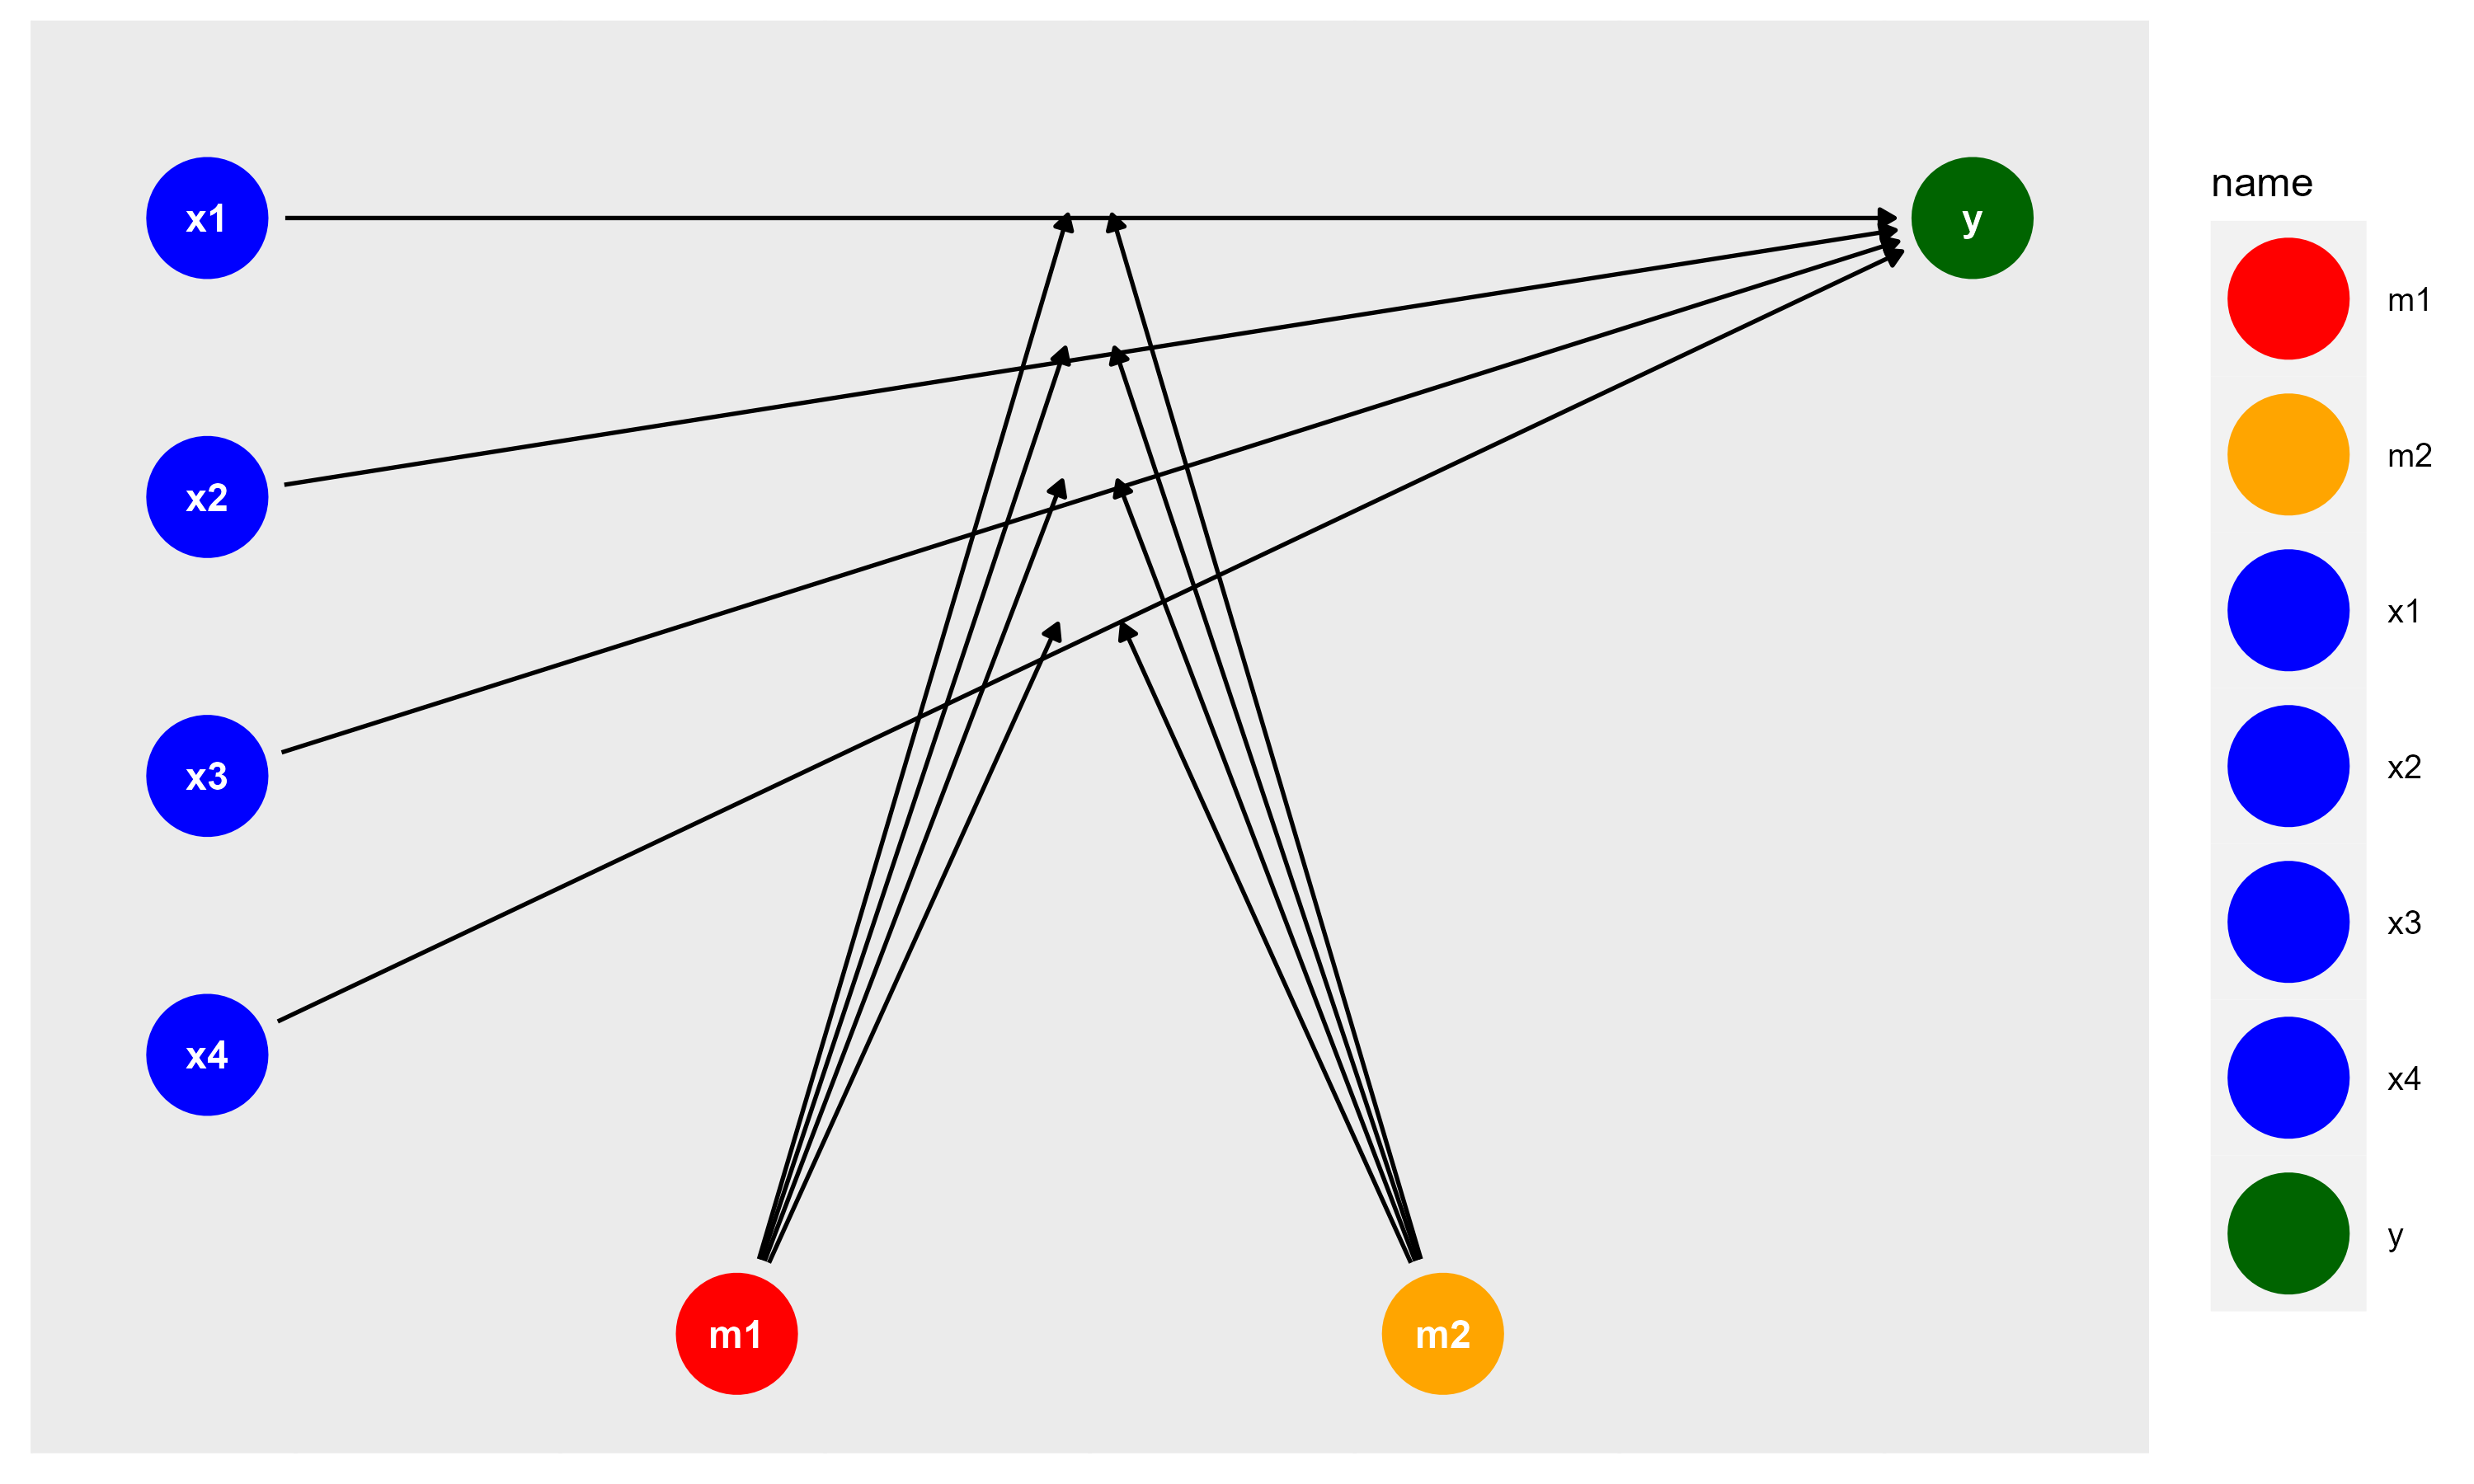
\includegraphics[width=0.5\textwidth,height=0.5\textheight]{C:/Users/danbo/OneDrive - Fundacao Getulio Vargas - FGV/FGV/Q3.23/GIT/GIT/dag_plot.png}
\caption{DAG: Moderators}\label{fig:label}
}
\end{figure}

\hypertarget{hypotheses-and-expected-results}{%
\subsection{Hypotheses and Expected
Results}\label{hypotheses-and-expected-results}}

In this section, we aim to provide insights into the expected outcomes
of our hypotheses by analyzing Table 2 together with Figure 5 and 6,
which illustrate the effects of framing on participants based on the
original experiment conducted by Healy \& Lenz (2014), which consider 25
hypothetical 4-year economies. In our experimental setup, participants
in the control condition will be exposed to yearly plots, while those in
the treatment condition viewed both yearly and cumulative (\(RDI_y\))
plots of 17 US presidential tenures from 1940 to 2008.

\begin{center}
  \begin{table}[!htbp]
\centering
\caption{Hypothetical Economies Framing Manipulation}

\begin{tabular}{@{\extracolsep{5pt}}lcccc}
\\[-1.8ex]\hline
\hline \\[-1.8ex]
\\[-1.8ex] & \multicolumn{1}{c}{Treatment 0} & \multicolumn{1}{c}{Treatment 1} & \multicolumn{1}{c}{Treatment 0 (Rescaled)} & \multicolumn{1}{c}{Treatment 1 (Rescaled)}  \\
\\[-1.8ex] & (1) & (2) & (3) & (4) \\
\hline \\[-1.8ex]
 RDI\textsubscript{1} & 0.124$^{*}$ & 0.436$^{***}$ & 0.021$^{*}$ & 0.069$^{***}$ \\
& (0.060) & (0.063) & (0.010) & (0.010) \\
 RDI\textsubscript{2} & 0.365$^{***}$ & 0.497$^{***}$ & 0.061$^{***}$ & 0.078$^{***}$ \\
& (0.053) & (0.056) & (0.009) & (0.009) \\
 RDI\textsubscript{3} & 0.462$^{***}$ & 0.545$^{***}$ & 0.077$^{***}$ & 0.086$^{***}$ \\
& (0.058) & (0.061) & (0.010) & (0.010) \\
 RDI\textsubscript{4} & 0.592$^{***}$ & 0.500$^{***}$ & 0.099$^{***}$ & 0.079$^{***}$ \\
& (0.040) & (0.042) & (0.007) & (0.007) \\
 const & 2.591$^{***}$ & 1.792$^{***}$ & -0.124$^{**}$ & -0.184$^{***}$ \\
& (0.286) & (0.302) & (0.048) & (0.048) \\
\hline \\[-1.8ex]
 Observations & 25 & 25 & 25 & 25 \\
 $R^2$ & 0.937 & 0.936 & 0.937 & 0.936 \\
 Adjusted $R^2$ & 0.925 & 0.923 & 0.925 & 0.923 \\
 Residual Std. Error & 0.468 (df=20) & 0.495 (df=20) & 0.078 (df=20) & 0.078 (df=20) \\
 F Statistic & 74.954$^{***}$ (df=4; 20) & 72.563$^{***}$ (df=4; 20) & 74.954$^{***}$ (df=4; 20) & 72.563$^{***}$ (df=4; 20) \\
\hline
\hline \\[-1.8ex]
\textit{Note:} & \multicolumn{4}{r}{$^{*}$p$<$0.1; $^{**}$p$<$0.05; $^{***}$p$<$0.01} \\
\end{tabular}
\end{table}
\end{center}

Table 2 depicts the relationship between respondents' economic
evaluations and income growth under such experimental conditions. For
participants framed with yearly growth information (Treatment 0), the
regression results reaffirm the patterns observed in the previous
analysis. (\(RDI_4\)) maintains a larger coefficient, underscoring its
influential role in shaping economic evaluations, and the associated
hypothesis tests validate the statistical significance of these
findings.

Notably, in the context of Treatment 1, where participants are exposed
to both yearly and cumulative growth information, the coefficients
exhibit a balanced distribution. Provided the additional information,
(\(RDI_4\)) no longer emerges as a key factor influencing economic
evaluations, demonstrating a clear change in the previous pattern.
Although, their hypothesis tests show a p-value less than 0.001 for the
case where participants observe only yearly growth and a p-value of
0.156 for the case where participants observe both cumulative and yearly
growth, authors find that for individual level regressions, the ratio of
the weight participants place on the fourth year relative to the first
decreases substantially, from 4.92 to 1.11 (p \textless{} 0.001).

\begin{figure}
\hypertarget{fig:label}{%
\centering
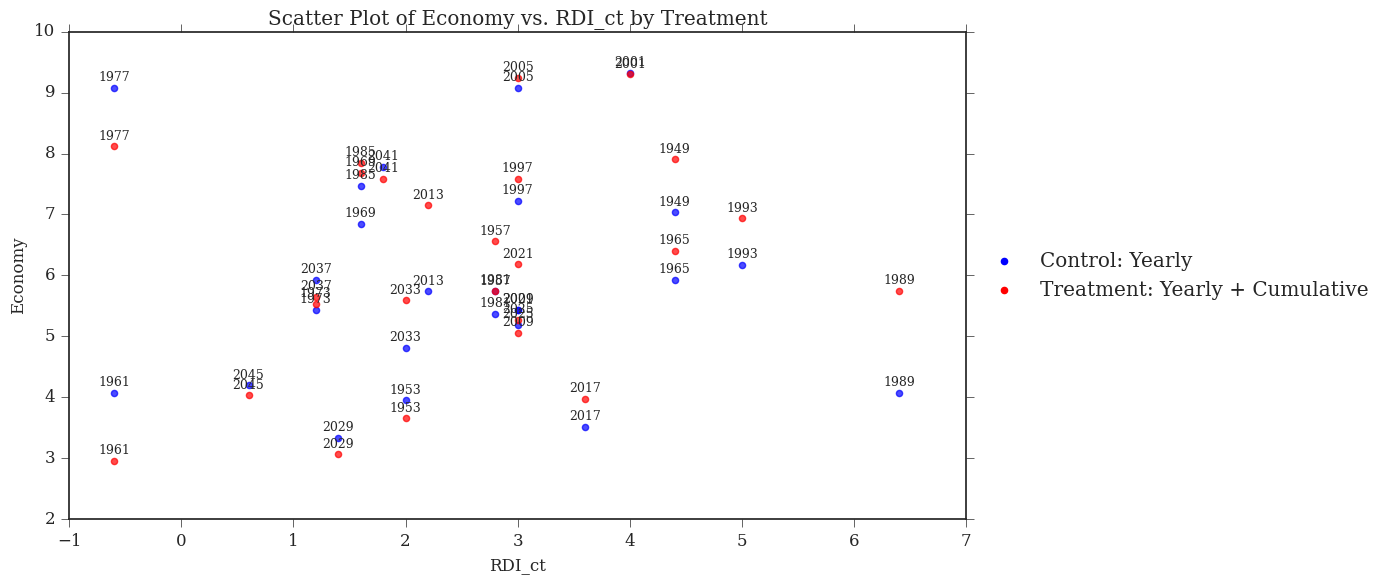
\includegraphics[width=1\textwidth,height=1\textheight]{difcuma.png}
\caption{Treatment Effect: Cross-Section}\label{fig:label}
}
\end{figure}

Figure 5 displays the combinations of economic evaluations (\(economy\))
and Election-Year Real Disposable Income Growth (\(RDI_y\)) of the 25
hypothetical economies, in a cross-sectional manner. It's evident that
the treatment rewards (punishes) economic evaluations, particularly at
the highest (lowest) ends of (\(RDI_y\)). For combinations characterized
by less extreme election-year growth values, we anticipate a milder yet
discernible effect. For a chronological perspective on this phenomenon,
please refer to Figure 6, which displays the hypothetical election-year
growth trends alongside economic evaluations for both control and
treatment conditions.

\begin{figure}
\hypertarget{fig:label}{%
\centering
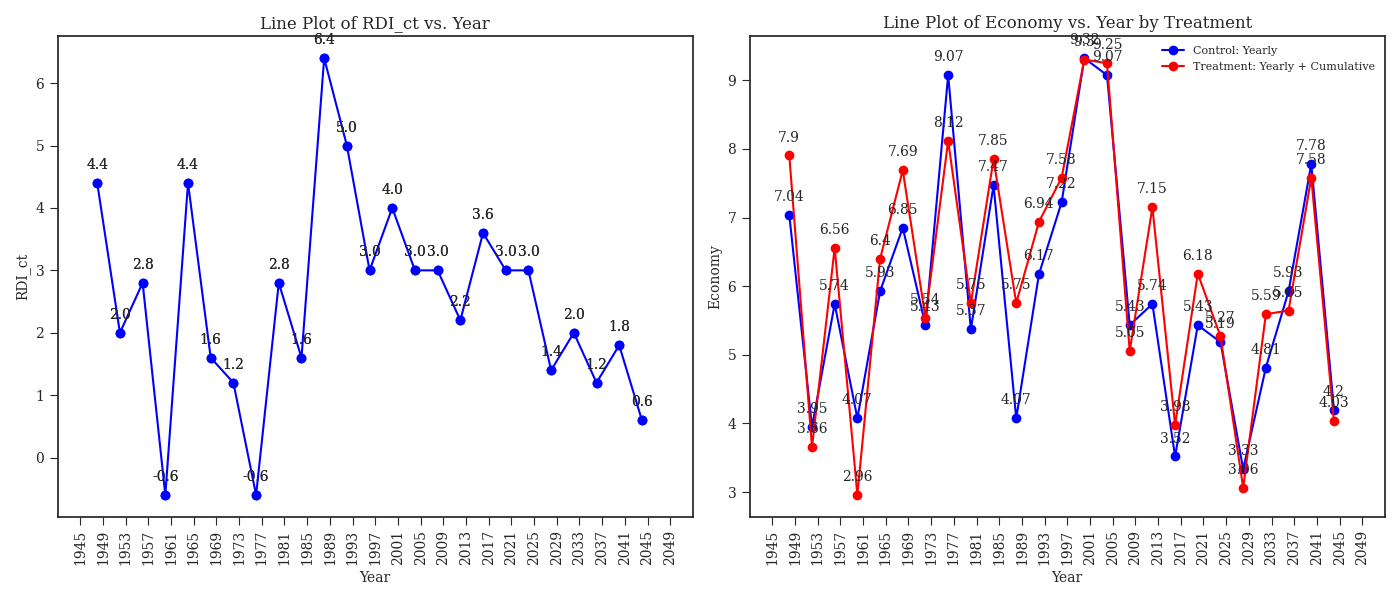
\includegraphics[width=1\textwidth,height=1\textheight]{difcum2.png}
\caption{Treatment Effect: Time-Series}\label{fig:label}
}
\end{figure}

The framing manipulation will involve presenting participants with real
economic data framed at either the yearly level (control condition) or
both the yearly and cumulative levels (treatment condition). This
manipulation will allow us to examine whether framing economic
information in a way that emphasizes both yearly and cumulative
performance helps participants to consider the entire term of an
incumbent, rather than just the election year. We expect that our
findings will align with the observations from the original experiment,
particularly for the Null Hypotheses.

\begin{itemize}
\tightlist
\item
  (\(H0 – Null\)): In the blind conditions, we expect that participants
  in the treatment condition will have more accurate and fair
  evaluations of the incumbent's economic performance than participants
  in the control condition. This is because framing the economic
  information in a way that emphasizes both yearly and cumulative
  performance will help them to consider the entire term of the
  incumbent, rather than just the election year.

  \begin{itemize}
  \tightlist
  \item
    In the control condition, participants will implicitly assign more
    weight to election-year growth. The first three coefficients will
    have small positive coefficients, while the fourth will be larger.
  \item
    In the treatment condition, participants will implicitly assign
    balanced weights to each of the four years.
  \end{itemize}
\end{itemize}

The affective manipulation will involve presenting participants with
real economic data for either an unidentified incumbent (blind
condition) or an identified incumbent (identified condition). This
manipulation will allow us to assess the impact of affective judgments
on participants' evaluations.

\begin{itemize}
\tightlist
\item
  (\(H1 – Affect-Driven\)): Our main hypothesis is that the mitigating
  effects found with the framing manipulation may not hold with real
  politicians towards whom respondents have prior affect.

  \begin{itemize}
  \tightlist
  \item
    In this case, if affect drives evaluations, there will be no
    relevant difference in judgments, regardless of whether individuals
    focus on election-year or cumulative economic performance.
  \item
    In the identified conditions, framing economic information may have
    a limited impact on voter myopia.
  \end{itemize}
\item
  (\(H2 – Mitigation\)): In the identified conditions, we expect that
  participants in the treatment condition will be less likely to be
  influenced by their affective judgments of the incumbent than
  participants in the control condition. This is because the additional
  information provided in the treatment condition will help them to make
  a more objective assessment of the incumbent's economic performance.

  \begin{itemize}
  \tightlist
  \item
    In the control condition, participants will implicitly assign more
    weight to election-year growth. The first three coefficients will
    have small positive coefficients, while the fourth will be larger.
    However, compared to the blind condition we expect more variance in
    the responses due to the influence of affective judgements.
  \item
    In the treatment condition, participants will implicitly assign
    balanced weights to each of the four years. However, compared to the
    control condition we expect less variance in the responses because
    of the mitigating effect of framing over the influence of affective
    judgements.
  \end{itemize}
\item
  (\(H3 – Backlash\)): Finally, we expect that the treatment effect will
  be larger (smaller) among participants who hold weak (strong) positive
  or negative affective judgments of the incumbent. This backlash is
  because individuals with stronger affective judgments are more likely
  to rationalize or resist information when making evaluations, whereas
  those with weaker affective judgements may be more receptive to new
  information.

  \begin{itemize}
  \tightlist
  \item
    In the identified treatment condition, participants with weak
    (strong) affective judgements will implicitly assign more (less)
    balanced weights to each of the four years.
  \end{itemize}
\end{itemize}

\begin{center}
  \begin{table}[!htbp]
\centering
\caption{Real Economies Framing and Affective Manipulation}

\begin{tabular}{@{\extracolsep{2pt}}lcccc}
\\[-1.8ex]\hline
\hline \\[-1.8ex]
\\[-1.8ex] & \multicolumn{1}{c}{Treatment 0 - Blind} & \multicolumn{1}{c}{Treatment 0 - Identified} & \multicolumn{1}{c}{Treatment 1 - Blind} & \multicolumn{1}{c}{Treatment 1 - Identified}  \\
\\[-1.8ex] & (1) & (2) & (3) & (4) \\
\hline \\[-1.8ex]
 RDI\textsubscript{1} & -0.020$^{*}$ & 0.015$^{}$ & 0.026$^{}$ & 0.032$^{}$ \\
& (0.010) & (0.022) & (0.024) & (0.025) \\
 RDI\textsubscript{2} & 0.026$^{**}$ & 0.002$^{}$ & -0.005$^{}$ & -0.004$^{}$ \\
& (0.010) & (0.022) & (0.024) & (0.025) \\
 RDI\textsubscript{3} & 0.080$^{***}$ & 0.047$^{}$ & 0.009$^{}$ & 0.007$^{}$ \\
& (0.013) & (0.029) & (0.032) & (0.034) \\
 RDI\textsubscript{4} & 0.131$^{***}$ & 0.104$^{***}$ & 0.047$^{}$ & 0.038$^{}$ \\
& (0.015) & (0.033) & (0.037) & (0.038) \\
 const & 0.101$^{*}$ & 0.056$^{}$ & 0.171$^{}$ & 0.236$^{}$ \\
& (0.053) & (0.118) & (0.131) & (0.137) \\
\hline \\[-1.8ex]
 Observations & 17 & 17 & 17 & 17 \\
 $R^2$ & 0.916 & 0.587 & 0.255 & 0.245 \\
 Adjusted $R^2$ & 0.888 & 0.449 & 0.006 & -0.007 \\
 Residual Std. Error & 0.102 (df=12) & 0.226 (df=12) & 0.251 (df=12) & 0.262 (df=12) \\
 F Statistic & 32.822$^{***}$ (df=4; 12) & 4.256$^{**}$ (df=4; 12) & 1.025$^{}$ (df=4; 12) & 0.973$^{}$ (df=4; 12) \\
\hline
\hline \\[-1.8ex]
\textit{Note:} & \multicolumn{4}{r}{$^{*}$p$<$0.1; $^{**}$p$<$0.05; $^{***}$p$<$0.01} \\
\end{tabular}
\end{table}
\end{center}

For the Null Hypothesis (\(H0\)) as displayed in Columns (1) and (3) of
Table 3, in control condition we expect the predicted values to converge
with the values of the original experiment. At a lower election-year
growth rate, the evaluations will cluster around the lower values of
economy, while at a higher election-year growth rate, they will
concentrate around the higher values. In the treatment condition, at a
lower cumulative growth rate, the evaluations will be punished with
respect to the evaluations in the control condition, and at a higher
cumulative growth rate, they will be rewarded with respect the
evaluations in the control condition. Figure 7 (left) displays the
extreme values while Figure 7 (right) displays the average effect around
the 33rd percentiles with blue bars for control and red for treatment
conditions.

\begin{figure}
\hypertarget{fig:label}{%
\centering
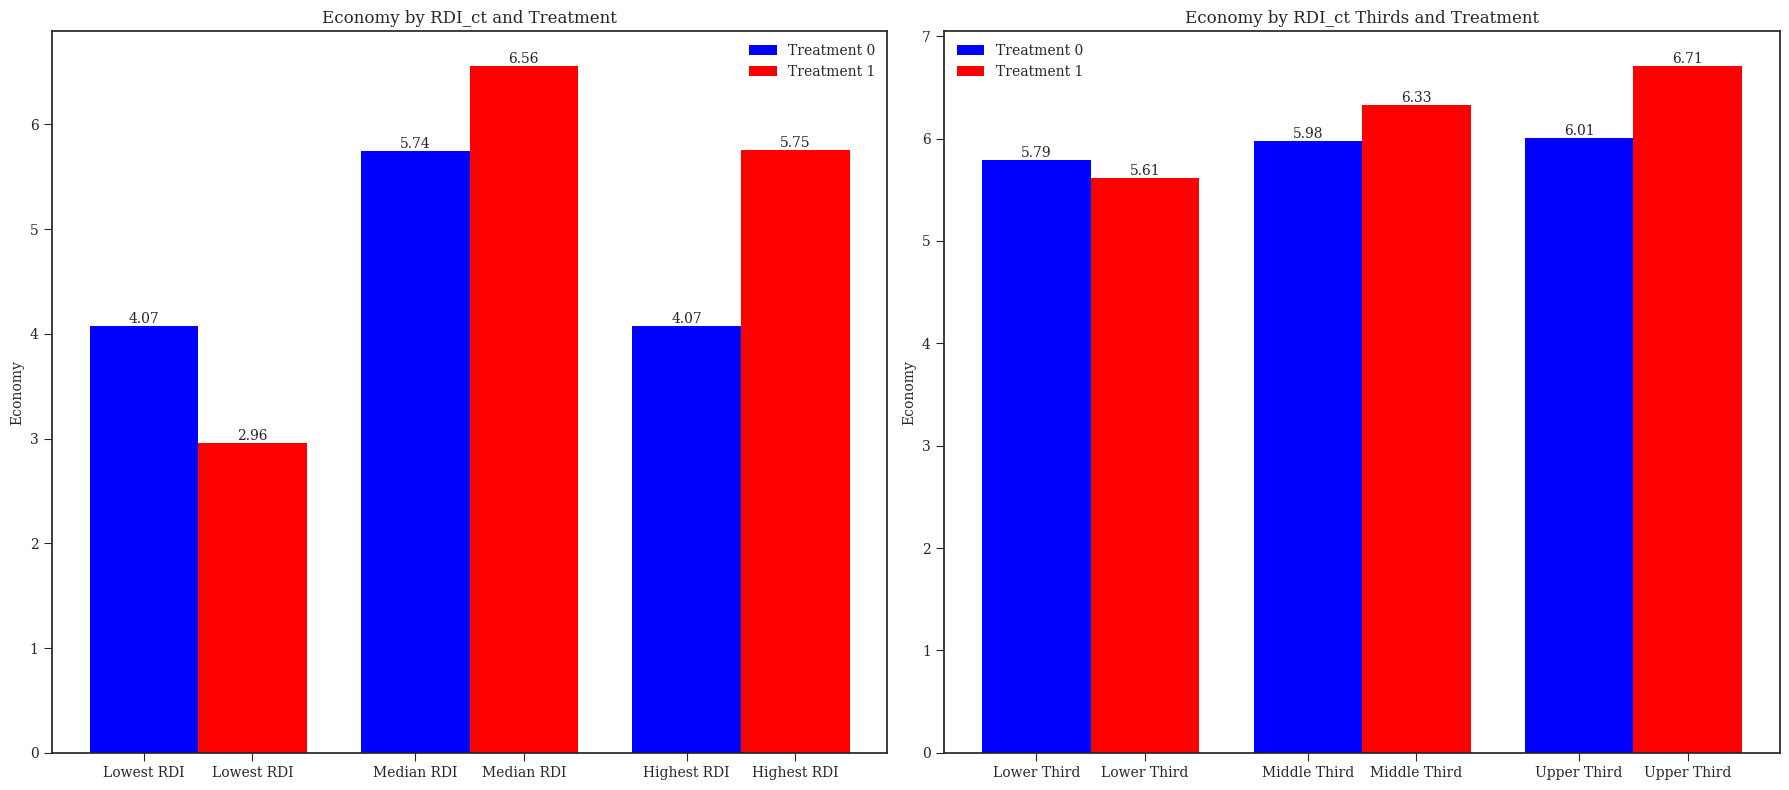
\includegraphics[width=1\textwidth,height=1\textheight]{treat_lowthird.png}
\caption{Hypothetical Economies Treatment Effects}\label{fig:label}
}
\end{figure}

Building on Campello \& Zucco (2022), we introduce presidents' names
into the individual (\(RDI\)) plots to test the affective treatment
condition. For the Affect-Driven Hypothesis (\(H1\)) we expect that the
mitigating effects found by Healy \& Lenz (2014) may not hold with real
politicians towards whom respondents have prior affect. If framing
economic information has limited impact on voter myopic behavior, there
will be no relevant difference in judgments, regardless of whether
individuals focus on election-year or cumulative economic performance.

For the Mitigation Hypothesis (\(H2\)) as displayed in Column (2) and
(4) of Table 3, with respect to the blind conditions, for the Identified
Control, we expect a larger effect on the evaluations caused by
participants affective judgements, while for the Identified Treatment a
smaller one. We expect the affective treatment to hold statistical
significance for values around the framing treatment, as displayed with
yellow bars in Figure 8. This outcome could provide compelling evidence
about the conditions when yearly and cumulative framing remain robust
even when participants can directly associate economic performance with
a president, effectively mitigating the end-bias and the influence of
prior affective judgments. For the Backlash Hypothesis (\(H3\)) results
will have to be detailed to consider the heterogeneity of participants
and their propensity to rationalize or update and embrace new or
challenging information.

\begin{figure}
\hypertarget{fig:label}{%
\centering
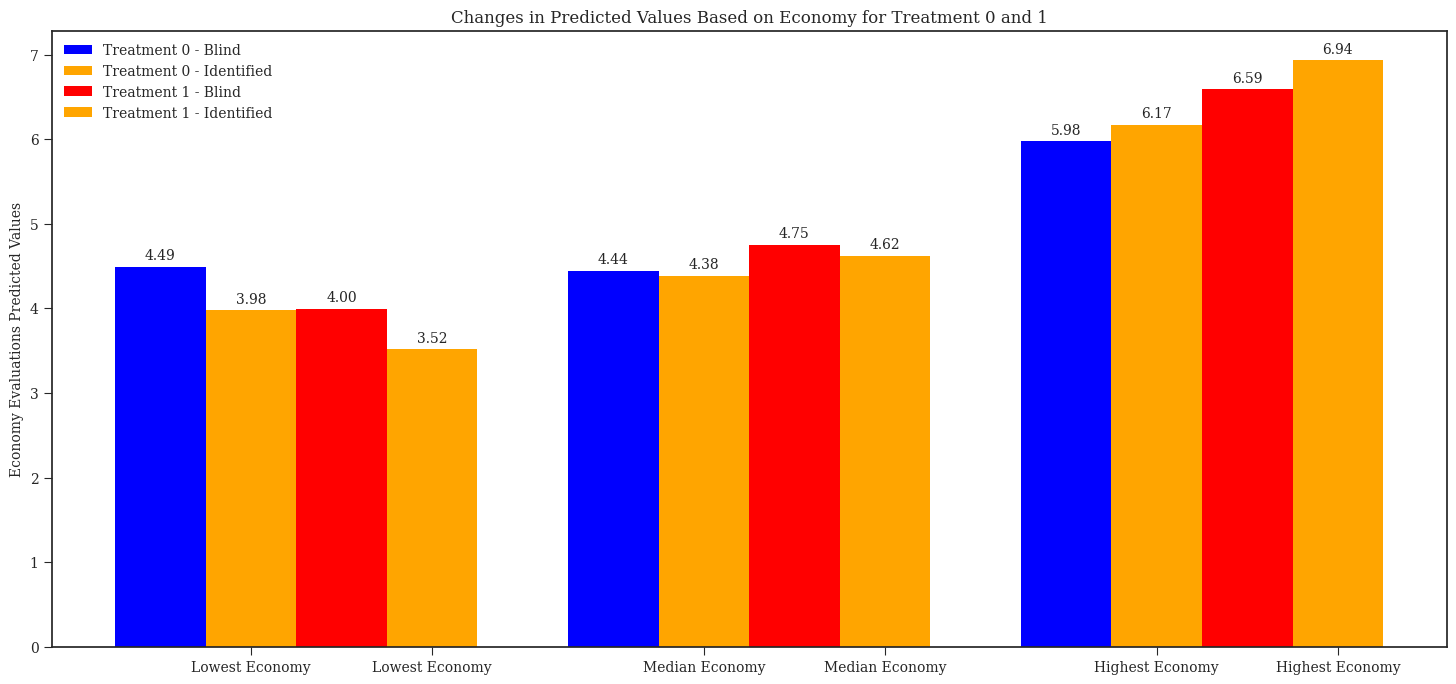
\includegraphics[width=1\textwidth,height=1\textheight]{pred_low.png}
\caption{Real Economies Predicted Treatment Effects}\label{fig:label}
}
\end{figure}

\hypertarget{why-this-matters}{%
\subsubsection{Why this matters}\label{why-this-matters}}

Framing offers a promising approach to counteract the end bias and
enhance the effectiveness of heuristics in political decision-making.
However, the presence of affective judgments and motivated reasoning
requires careful consideration of framing techniques to ensure that
citizens overcome myopic behaviors in order to make balanced and
informed choices, ultimately reinforcing democratic accountability. It
is necessary to explore whether voters respond to government performance
and if they do so in a manner that aligns their actions with their
intentions. While implementing these changes in real-world settings
poses challenges, acknowledging the cognitive underpinnings of this
phenomenon could open the door to relatively simple modifications in the
information context, such as emphasizing cumulative growth.

\hypertarget{results-of-the-online-experiments-tbd}{%
\subsection{\texorpdfstring{Results of the Online Experiments
\emph{{[}TBD{]}}}{Results of the Online Experiments {[}TBD{]}}}\label{results-of-the-online-experiments-tbd}}

\hypertarget{implications-limitations-and-future-research-tbd}{%
\subsection{\texorpdfstring{Implications, Limitations, and Future
Research
\emph{{[}TBD{]}}}{Implications, Limitations, and Future Research {[}TBD{]}}}\label{implications-limitations-and-future-research-tbd}}

\hypertarget{discussion-and-conclusion-tbd}{%
\subsection{\texorpdfstring{Discussion and Conclusion
\emph{{[}TBD{]}}}{Discussion and Conclusion {[}TBD{]}}}\label{discussion-and-conclusion-tbd}}

\singlespacing

\hypertarget{references}{%
\subsection{References}\label{references}}

\hypertarget{refs}{}
\begin{CSLReferences}{1}{0}
\leavevmode\vadjust pre{\hypertarget{ref-achenbartels_2004}{}}%
Achen, C. H., \& Bartels, L. M. (2004). \emph{Musical {Chairs}:
{Pocketbook Voting} and the {Limits} of {Democratic Accountability}}.

\leavevmode\vadjust pre{\hypertarget{ref-bartels_1996}{}}%
Bartels, L. M. (1996). Uninformed {Votes}: {Information Effects} in
{Presidential Elections}. \emph{American Journal of Political Science},
\emph{40}(1), 194--230. \url{https://doi.org/10.2307/2111700}

\leavevmode\vadjust pre{\hypertarget{ref-Baumgarten_1997}{}}%
Baumgartner, H., Sujan, M., \& Padgett, D. (1997). Patterns of
{Affective Reactions} to {Advertisements}: {The Integration} of
{Moment-to-Moment Responses} into {Overall Judgments}. \emph{Journal of
Marketing Research}, \emph{Vol. XXXIV}.

\leavevmode\vadjust pre{\hypertarget{ref-camzuvol_2020}{}}%
Campello, D., \& Zucco, C. (2020). \emph{The {Volatility Curse}:
{Exogenous Shocks} and {Representation} in {Resource-Rich Democracies}}.
{Cambridge University Press}.
\url{https://doi.org/10.1017/9781108894975}

\leavevmode\vadjust pre{\hypertarget{ref-CampelloZucco_CommodityPrices2022}{}}%
Campello, D., \& Zucco, C. (2022). \emph{Commodity {Prices}, {Relative
Performance}, and {Misattribution} of {Responsibility} for the
{Economy}}.

\leavevmode\vadjust pre{\hypertarget{ref-ohpp_chong_2013}{}}%
Chong, D. (2013). Degrees of {Rationality} in {Politics}. In L. Huddy,
D. O. Sears, \& J. S. Levy (Eds.), \emph{The {Oxford Handbook} of
{Political Psychology}} (p. 0). {Oxford University Press}.
\url{https://doi.org/10.1093/oxfordhb/9780199760107.013.0004}

\leavevmode\vadjust pre{\hypertarget{ref-downs_1957}{}}%
Downs, A. (1957). \emph{An {Economic Theory} of {Democracy}}. {Harper}.

\leavevmode\vadjust pre{\hypertarget{ref-druckman_2001}{}}%
Druckman, J. N. (2001a). On the {Limits} of {Framing Effects}: {Who Can
Frame}? \emph{The Journal of Politics}, \emph{63}(4), 1041--1066.
\url{https://www.jstor.org/stable/2691806}

\leavevmode\vadjust pre{\hypertarget{ref-druckman_2001b}{}}%
Druckman, J. N. (2001b). The {Implications} of {Framing Effects} for
{Citizen Competence}. \emph{Political Behavior}, \emph{23}(3), 225--256.
\url{https://doi.org/10.1023/A:1015006907312}

\leavevmode\vadjust pre{\hypertarget{ref-fair_1978}{}}%
Fair, R. C. (1978). The {Effect} of {Economic Events} on {Votes} for
{President}. \emph{The Review of Economics and Statistics},
\emph{60}(2), 159. \url{https://doi.org/10.2307/1924969}

\leavevmode\vadjust pre{\hypertarget{ref-fiorina_1981}{}}%
Fiorina, M. P. (1981). \emph{Retrospective {Voting} in {American
National Elections}}. {Yale University Press}.

\leavevmode\vadjust pre{\hypertarget{ref-Goffman_1986}{}}%
Goffman, E. (1986). \emph{Frame analysis: An essay on the organization
of experience} (Northeastern University Press ed). {Northeastern
University Press}.

\leavevmode\vadjust pre{\hypertarget{ref-HealyLenz_2014}{}}%
Healy, A., \& Lenz, G. S. (2014). Substituting the {End} for the
{Whole}: {Why Voters Respond Primarily} to the {Election-Year Economy}.
\emph{American Journal of Political Science}, \emph{58}(1), 31--47.
\url{https://doi.org/10.1111/ajps.12053}

\leavevmode\vadjust pre{\hypertarget{ref-huhilenz_2012}{}}%
Huber, G. A., Hill, S. J., \& Lenz, G. S. (2012). Sources of {Bias} in
{Retrospective Decision Making}: {Experimental Evidence} on {Voters}'
{Limitations} in {Controlling Incumbents}. \emph{American Political
Science Review}, \emph{106}(4), 720--741.
\url{https://doi.org/10.1017/S0003055412000391}

\leavevmode\vadjust pre{\hypertarget{ref-kahn_2003}{}}%
Kahneman, D. (2003). Maps of {Bounded Rationality}: {Psychology} for
{Behavioral Economics}. \emph{American Economic Review}, \emph{93}(5),
1449--1475. \url{https://doi.org/10.1257/000282803322655392}

\leavevmode\vadjust pre{\hypertarget{ref-kahn_2011}{}}%
Kahneman, D. (2011). \emph{Thinking, {Fast} and {Slow}}. {Farrar, Straus
and Giroux}.

\leavevmode\vadjust pre{\hypertarget{ref-kahntev_1979}{}}%
Kahneman, D., \& Tversky, A. (1979). Prospect {Theory}: {An Analysis} of
{Decision} under {Risk}. \emph{Econometrica}, \emph{47}(2), 263--291.
\url{https://doi.org/10.2307/1914185}

\leavevmode\vadjust pre{\hypertarget{ref-key_1966}{}}%
Key, V. O. J. (1966). \emph{The {Responsible Electorate}: {Rationality}
in {Presidential Voting}, 1936{\textendash}1960}. {Belknap Press}.

\leavevmode\vadjust pre{\hypertarget{ref-kramer_1971}{}}%
Kramer, G. H. (1971). Short-{Term Fluctuations} in {U}.{S}. {Voting
Behavior}, 1896{\textendash}1964. \emph{American Political Science
Review}, \emph{65}(1), 131--143. \url{https://doi.org/10.2307/1955049}

\leavevmode\vadjust pre{\hypertarget{ref-kukquirk_2000}{}}%
Kuklinski, J. H., \& Quirk, P. J. (2000). Reconsidering the {Rational
Public}: {Cognition}, {Heuristics}, and {Mass Opinion}. In A. Lupia, M.
D. McCubbins, \& S. L. Popkin (Eds.), \emph{Elements of {Reason}:
{Cognition}, {Choice}, and the {Bounds} of {Rationality}} (pp.
153--182). {Cambridge University Press}.
\url{https://doi.org/10.1017/CBO9780511805813.008}

\leavevmode\vadjust pre{\hypertarget{ref-Lakoff_2014}{}}%
Lakoff, G. (2014). \emph{The all-new don't think of an elephant! Know
your values and frame the debate}. {Chelsea Green Publishing}.

\leavevmode\vadjust pre{\hypertarget{ref-redlau_1997}{}}%
Lau, R. R., \& Redlawsk, D. P. (1997). {Voting correctly}.
\emph{American Political Science Review}, \emph{91}(3), 585--598.
\url{https://doi.org/10.2307/2952076}

\leavevmode\vadjust pre{\hypertarget{ref-redlau_2001}{}}%
Lau, R. R., \& Redlawsk, D. P. (2001). {Advantages and disadvantages of
cognitive heuristics in political decision making}. \emph{American
journal of political science}, \emph{45}(4), 951--971.
\url{https://doi.org/10.2307/2669334}

\leavevmode\vadjust pre{\hypertarget{ref-taberlodge_2005}{}}%
Lodge, M., \& Taber, C. S. (2005). The {Automaticity} of {Affect} for
{Political Leaders}, {Groups}, and {Issues}: {An Experimental Test} of
the {Hot Cognition Hypothesis}. \emph{Political Psychology},
\emph{26}(3), 455--482.
\url{https://doi.org/10.1111/j.1467-9221.2005.00426.x}

\leavevmode\vadjust pre{\hypertarget{ref-taberlodge_2013}{}}%
Lodge, M., \& Taber, C. S. (2013). \emph{The {Rationalizing Voter}}.
{Cambridge University Press}.

\leavevmode\vadjust pre{\hypertarget{ref-Neuman_2000}{}}%
Marcus, G. E., Neuman, W. R., \& MacKuen, M. (2000). \emph{Affective
intelligence and political judgment}. {University of Chicago Press}.

\leavevmode\vadjust pre{\hypertarget{ref-McCombs_1972}{}}%
McCombs, M. E., \& Shaw, D. L. (1972). The {Agenda-Setting Function} of
{Mass Media}. \emph{The Public Opinion Quarterly}, \emph{36}(2),
176--187. \url{https://www.jstor.org/stable/2747787}

\leavevmode\vadjust pre{\hypertarget{ref-vonneumorg_1947}{}}%
Neumann, J. von, \& Morgenstern, O. (2007). \emph{Theory of {Games} and
{Economic Behavior}: 60th {Anniversary Commemorative Edition}}.
{Princeton University Press}.

\leavevmode\vadjust pre{\hypertarget{ref-redkahn_1996}{}}%
Redelmeier, D. A., \& Kahneman, D. (1996). Patients' memories of painful
medical treatments: Real-time and retrospective evaluations of two
minimally invasive procedures. \emph{Pain}, \emph{66}(1), 3--8.
\url{https://doi.org/10.1016/0304-3959(96)02994-6}

\leavevmode\vadjust pre{\hypertarget{ref-ohpp_redlau_2013}{}}%
Redlawsk, D. P., \& Lau, R. R. (2013). Behavioral {Decision-Making}. In
L. Huddy, D. O. Sears, \& J. S. Levy (Eds.), \emph{The {Oxford Handbook}
of {Political Psychology}} (p. 0). {Oxford University Press}.
\url{https://doi.org/10.1093/oxfordhb/9780199760107.013.0005}

\leavevmode\vadjust pre{\hypertarget{ref-simon_1957}{}}%
Simon, H. A. (1957). \emph{Models of {Man}: {Social} and {Rational};
{Mathematical Essays} on {Rational Human Behavior} in {Society
Setting}}. {Wiley}.

\leavevmode\vadjust pre{\hypertarget{ref-Sniderman_2004}{}}%
Sniderman, P. M., \& Theriault, S. M. (2004). \emph{The {Structure} of
{Political Argument} and the {Logic} of {Issue Framing}}.

\leavevmode\vadjust pre{\hypertarget{ref-ohpp_taberlodge_2013}{}}%
Taber, C. S., \& Young, E. (2013). Political {Information Processing}.
In L. Huddy, D. O. Sears, \& J. S. Levy (Eds.), \emph{The {Oxford
Handbook} of {Political Psychology}} (p. 0). {Oxford University Press}.
\url{https://doi.org/10.1093/oxfordhb/9780199760107.013.0017}

\leavevmode\vadjust pre{\hypertarget{ref-tufte_1978}{}}%
Tufte, E. R. (1978). \emph{Political control of the economy} (1.
Paperback ed). {Princeton Univ. Press}.

\leavevmode\vadjust pre{\hypertarget{ref-tvekahn_1974}{}}%
Tversky, A., \& Kahneman, D. (1974). Judgment under uncertainty:
{Heuristics} and biases. \emph{Science}, \emph{185}(4157), 1124--1131.
\url{https://doi.org/10.1126/science.185.4157.1124}

\end{CSLReferences}

\newpage

\hypertarget{annex}{%
\subsection{Annex}\label{annex}}

\hypertarget{github}{%
\subsubsection{Github}\label{github}}

Online version can be accessed at this
\href{https://danybonfil.github.io/start/}{\textbf{Github Repository}}

\hypertarget{survey-details}{%
\subsubsection{Survey Details}\label{survey-details}}

Survey can be accessed at this
\href{https://survey.fgv.br/jfe/form/SV_5jUiMOHHgM1t0DY}{\textbf{Qualtrics
Link}}

\begin{figure}
\hypertarget{fig:label}{%
\centering
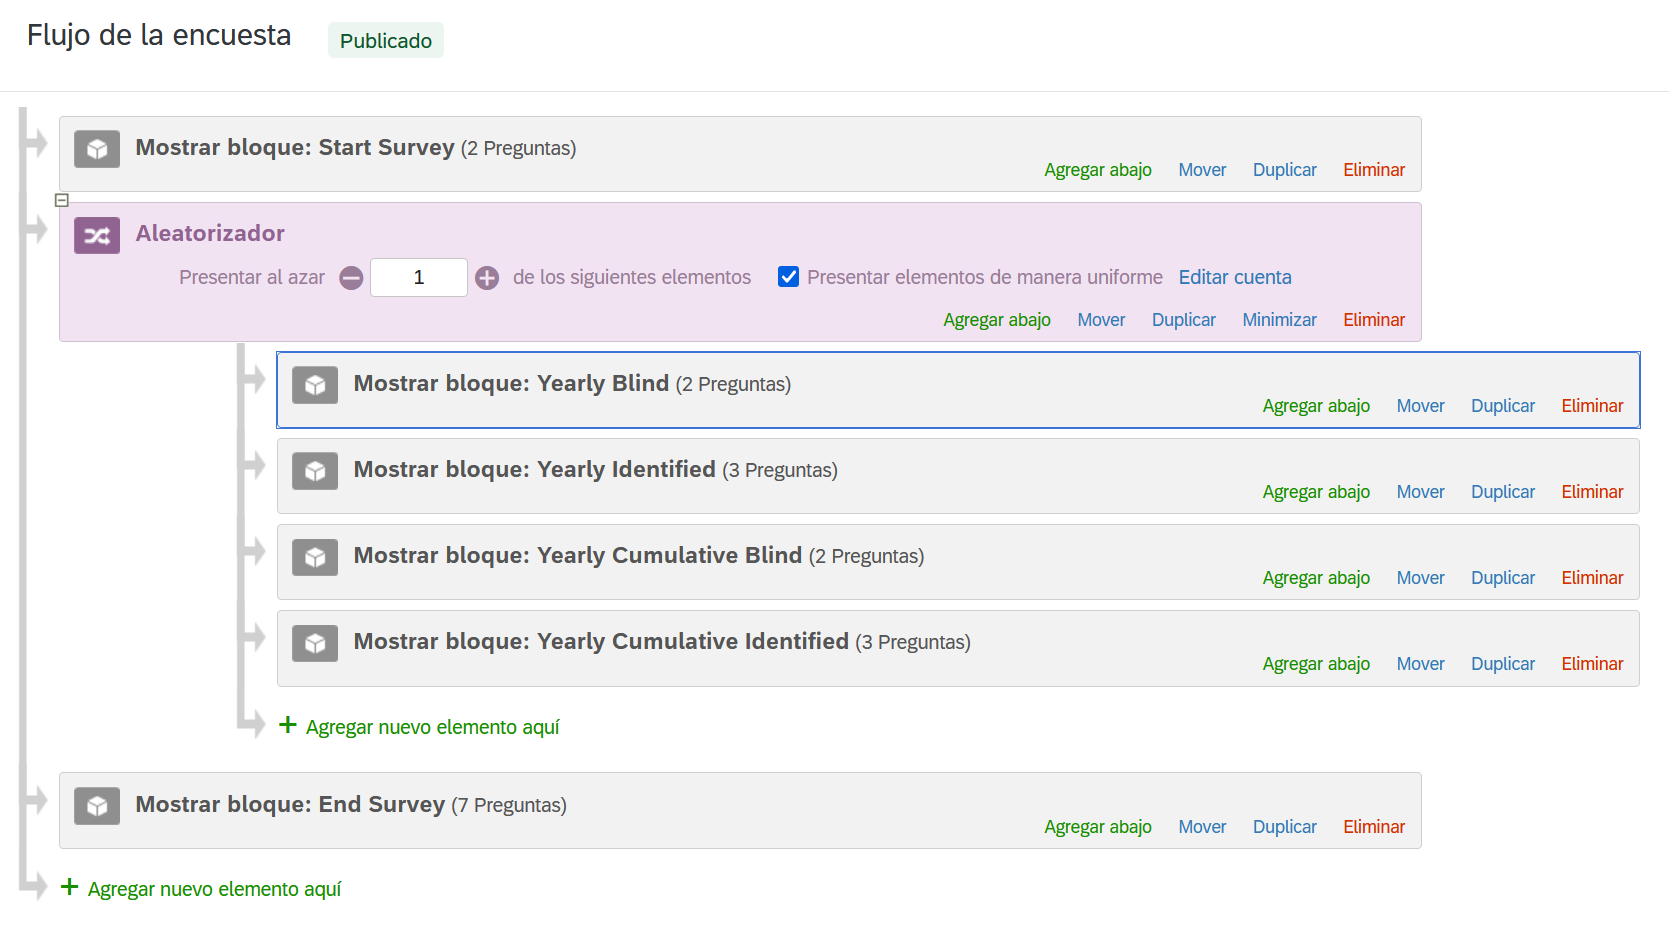
\includegraphics[width=1\textwidth,height=1\textheight]{flow_survey.png}
\caption{Survey Flow}\label{fig:label}
}
\end{figure}

\begin{figure}
\hypertarget{fig:label}{%
\centering
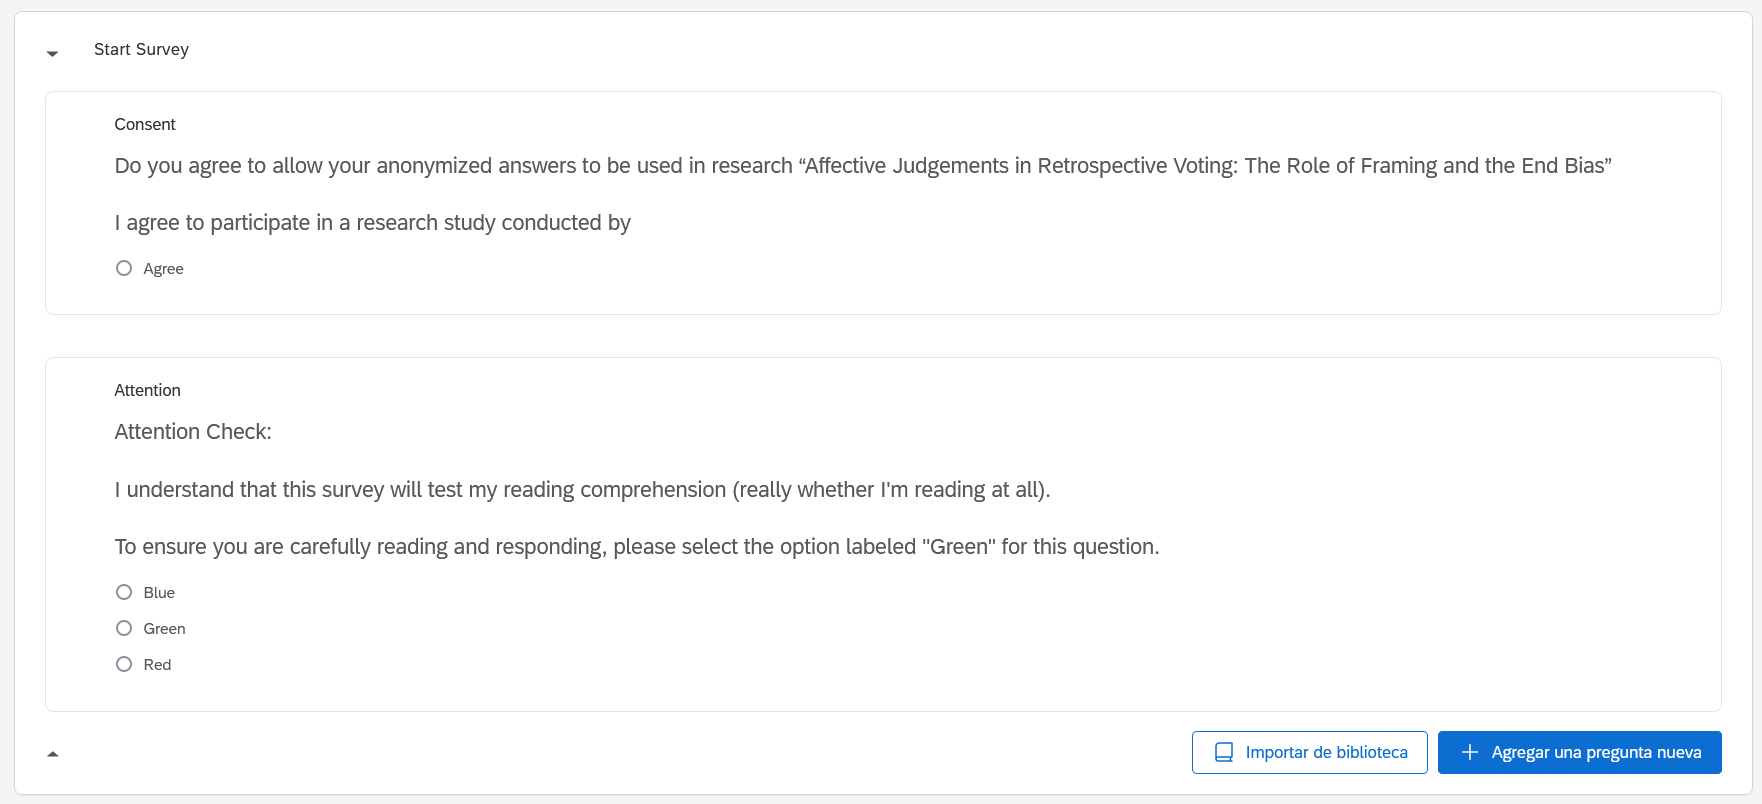
\includegraphics[width=1\textwidth,height=1\textheight]{start_survey.png}
\caption{Start Survey}\label{fig:label}
}
\end{figure}

\begin{figure}
\hypertarget{fig:label}{%
\centering
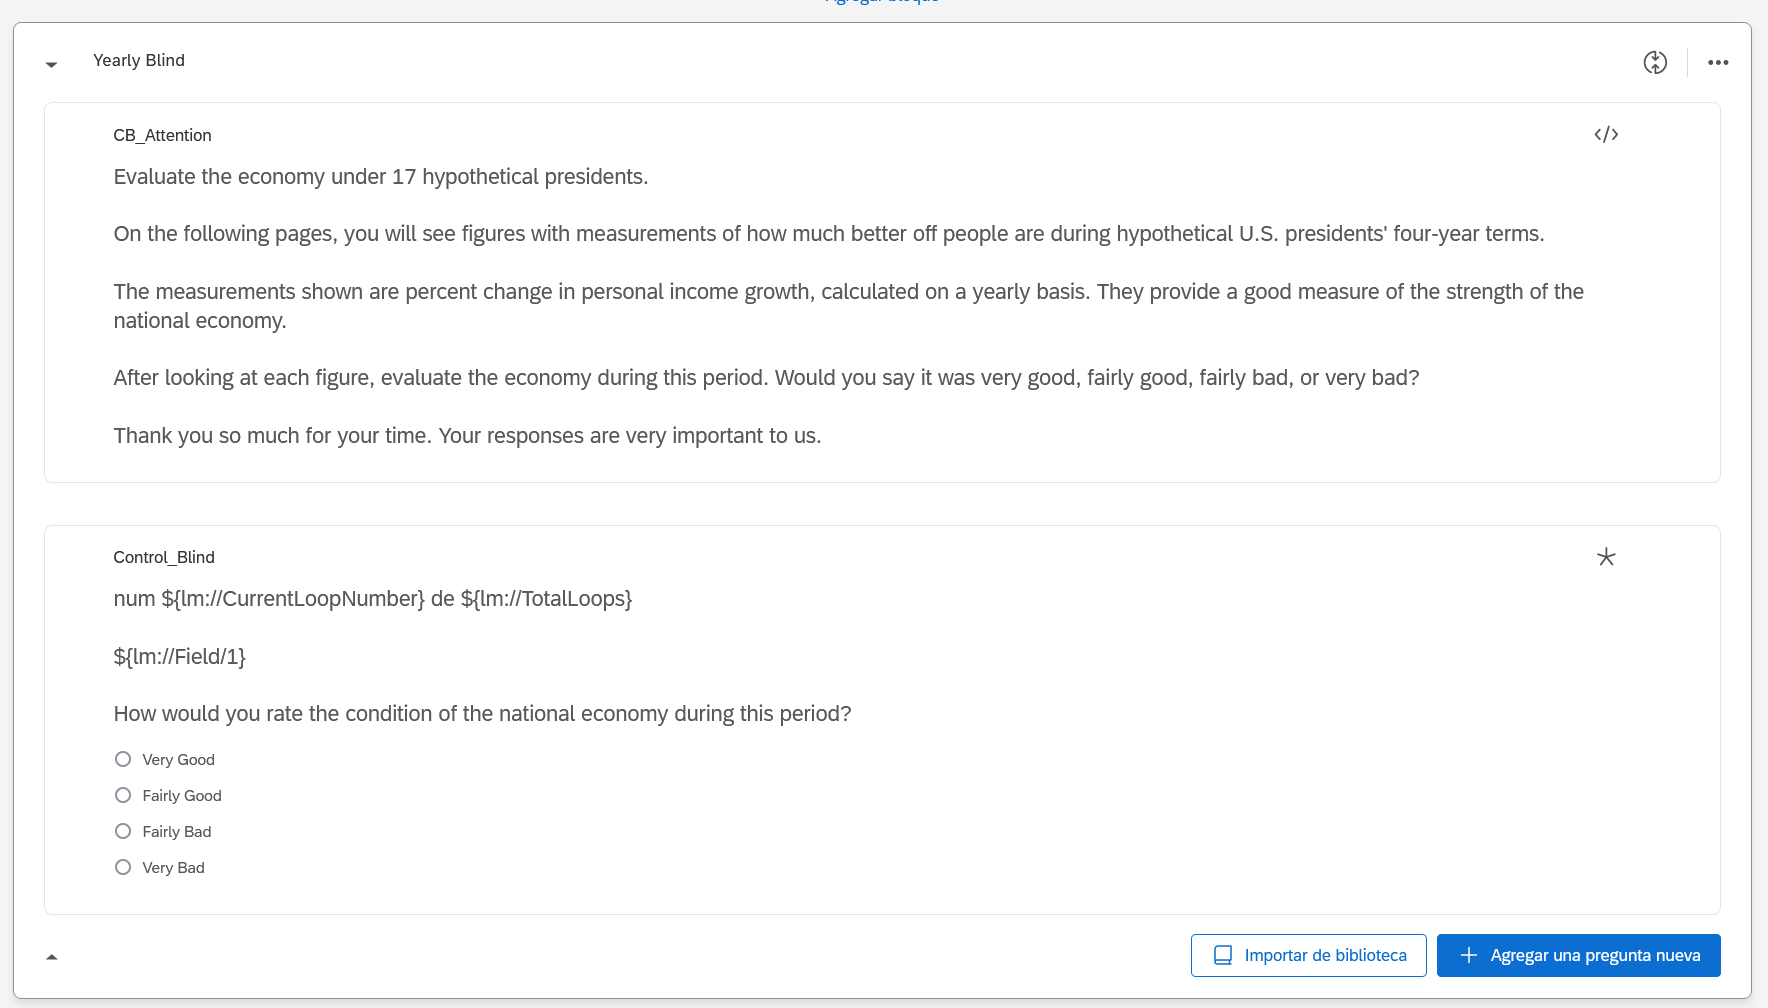
\includegraphics[width=1\textwidth,height=1\textheight]{control_blind.png}
\caption{Control Blind}\label{fig:label}
}
\end{figure}

\begin{figure}
\hypertarget{fig:label}{%
\centering
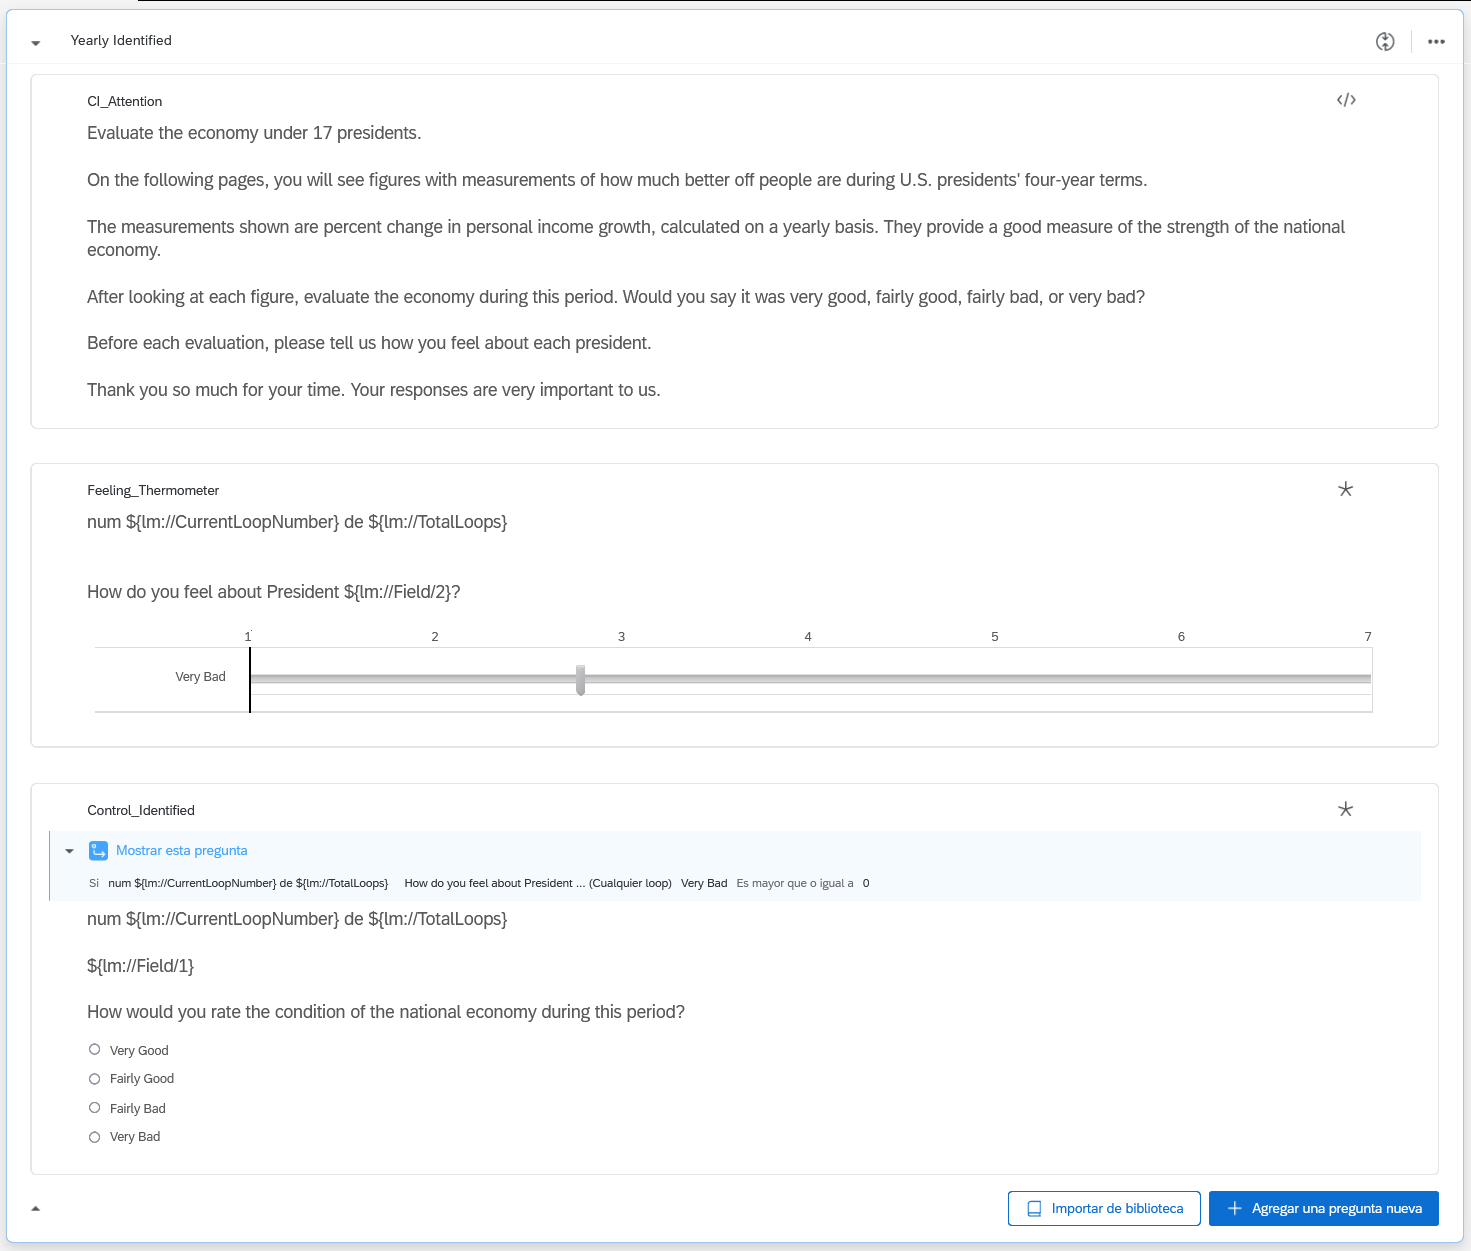
\includegraphics[width=1\textwidth,height=1\textheight]{control_identified.png}
\caption{Control Identified}\label{fig:label}
}
\end{figure}

\begin{figure}
\hypertarget{fig:label}{%
\centering
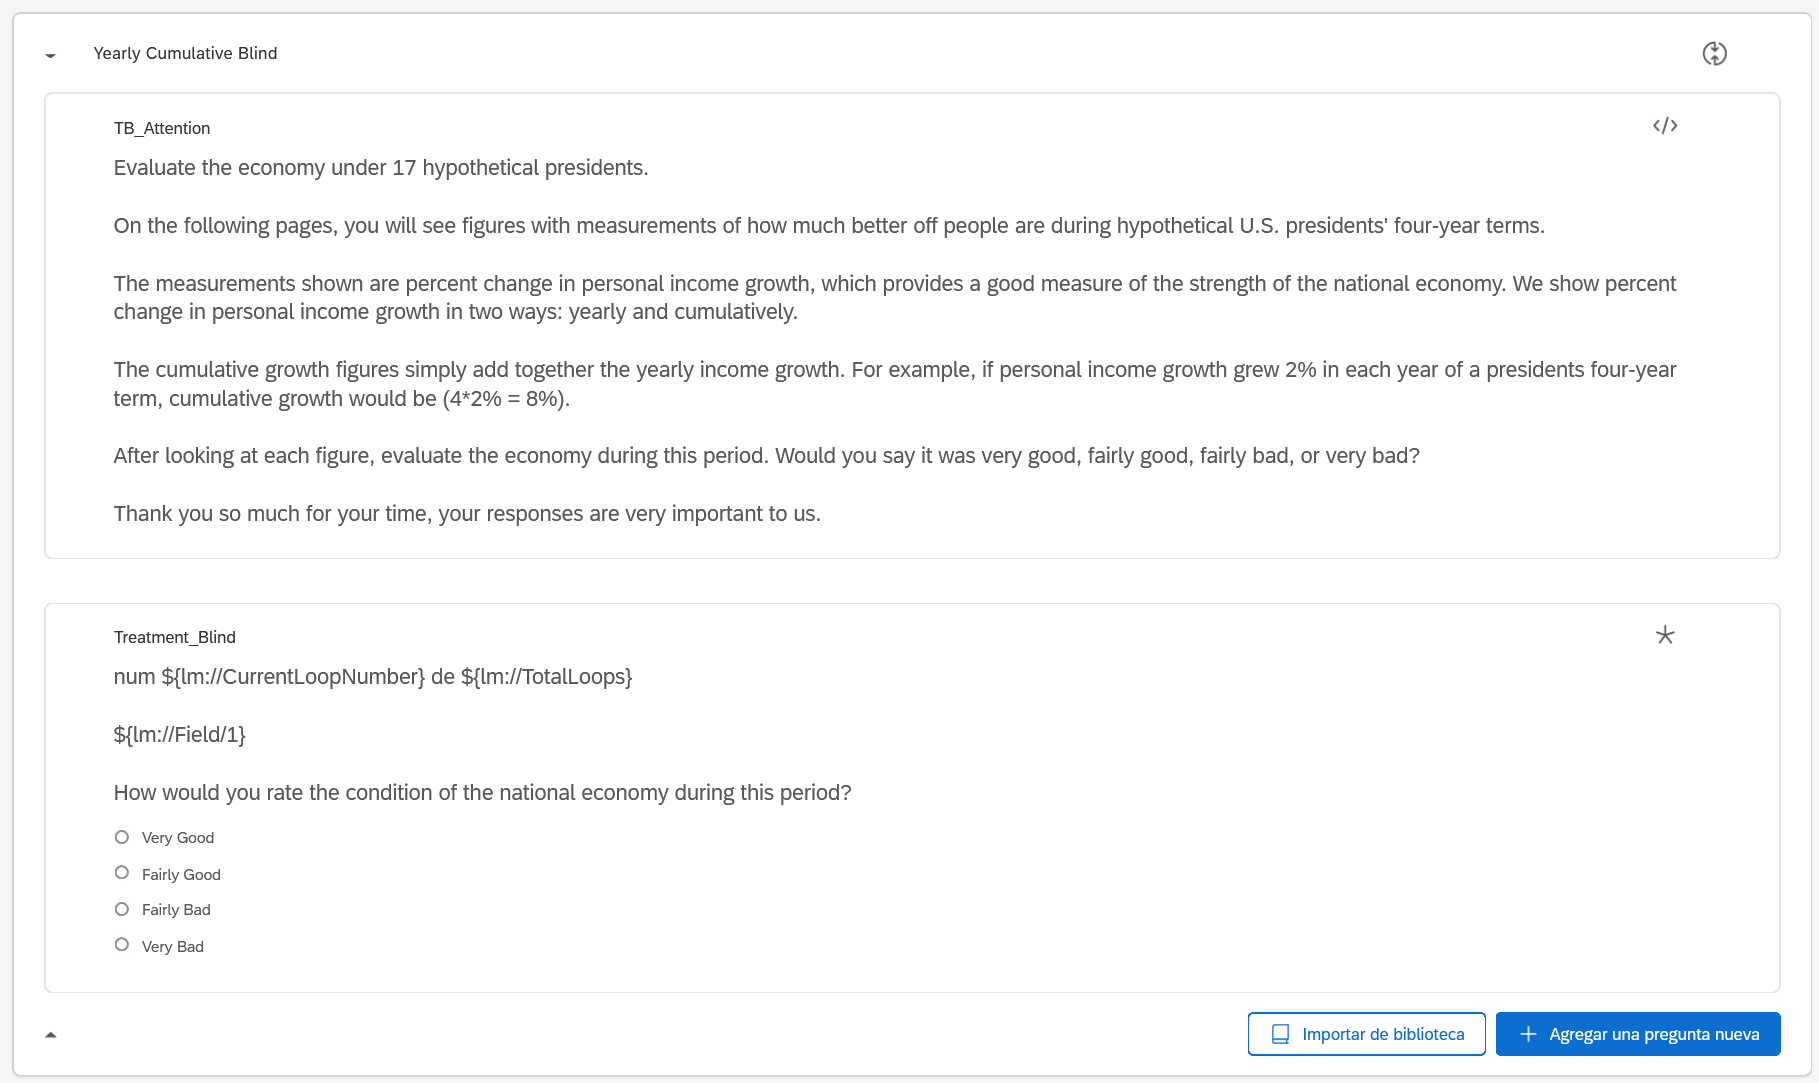
\includegraphics[width=1\textwidth,height=1\textheight]{treat_blind.png}
\caption{Treatment Blind}\label{fig:label}
}
\end{figure}

\begin{figure}
\hypertarget{fig:label}{%
\centering
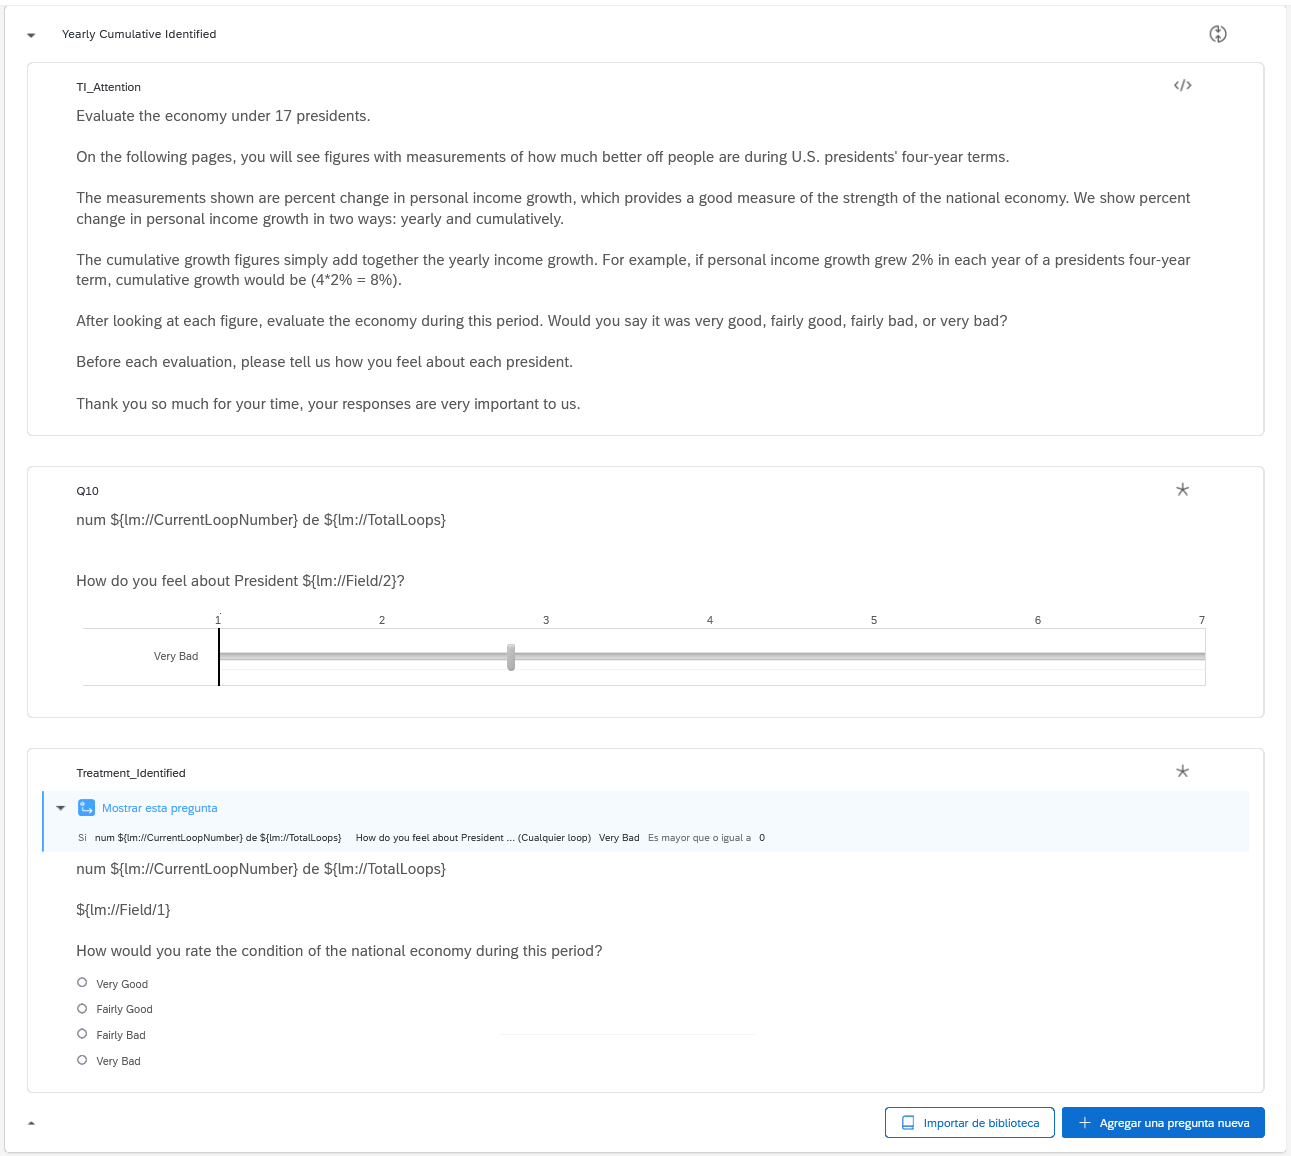
\includegraphics[width=1\textwidth,height=1\textheight]{treat_identified.png}
\caption{Treatment Identified}\label{fig:label}
}
\end{figure}

\begin{figure}
\hypertarget{fig:label}{%
\centering
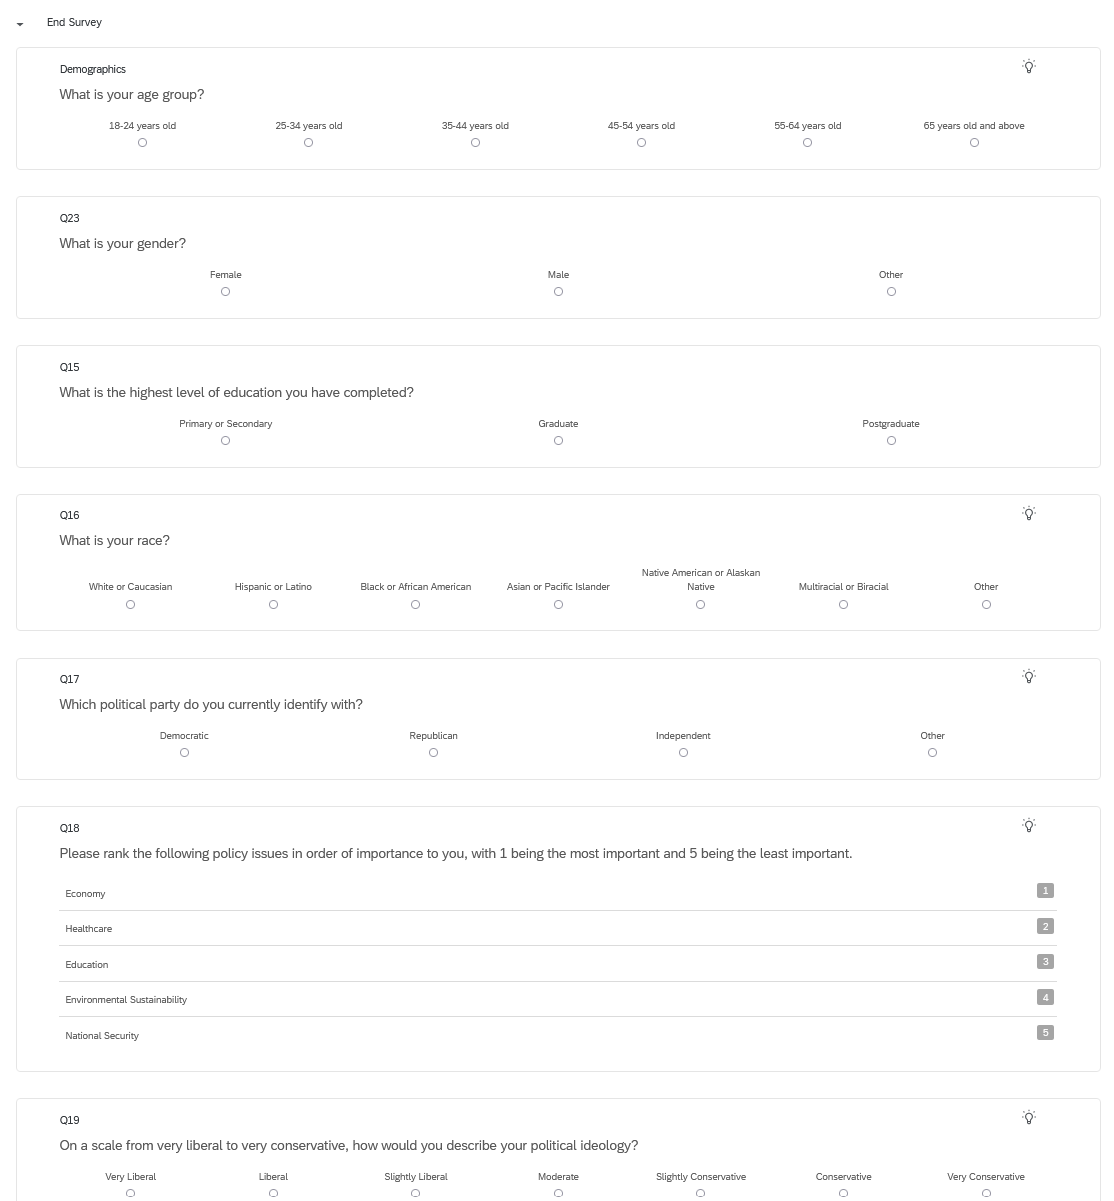
\includegraphics[width=1\textwidth,height=1\textheight]{end_survey.png}
\caption{End Survey}\label{fig:label}
}
\end{figure}

\end{document}
